\documentclass[12pt,fleqn]{book} % Default font size and left-justified equations
\renewcommand{\baselinestretch}{1.65}
%----------------------------------------------------------------------------------------

%----------------------------------------------------------------------------------------
%	VARIOUS REQUIRED PACKAGES
%----------------------------------------------------------------------------------------

\usepackage[top=2.5cm,bottom=2.5cm,left=3cm,right=3cm,headsep=10pt,a4paper]{geometry} % Page margins
\usepackage{titlesec} % Allows customization of titles
\usepackage{tcolorbox}
\usepackage{multicol}
\everymath{\displaystyle}
\usepackage{graphicx} % Required for including pictures
\graphicspath{{Pictures/}} % Specifies the directory where pictures are stored

\usepackage{lipsum} % Inserts dummy text

\usepackage{tikz} % Required for drawing custom shapes

\usepackage[english]{babel} % English language/hyphenation

\usepackage{enumitem} % Customize lists
\setlist{nolistsep} % Reduce spacing between bullet points and numbered lists

\usepackage{booktabs} % Required for nicer horizontal rules in tables

\usepackage{eso-pic} % Required for specifying an image background in the title page

\usepackage{xcolor} % Required for specifying colors by name
\definecolor{ocre}{RGB}{51,102,0} 
\definecolor{lightgray}{RGB}{229,229,229}  % Define the orange color used for highlighting throughout the book
%--------------------------------------------------------------------------------------------------------------------------------
%%%% khmer cod 
%-------------------------------------------------------------------------------------------------------------------------------
\usepackage{fontspec}  
\usepackage{xltxtra}
\defaultfontfeatures{Mapping=tex-text}
\XeTeXlinebreaklocale "khm"
\XeTeXlinebreakskip = 0pt plus 1pt minus 1pt 
\setmainfont [Scale = 0.8333333334, Script=Khmer]{Khmer OS Battambang}
\setmathrm{Times New Roman}
\newcommand{\ko}{\fontspec[Scale = 0.8333333334, Script=Khmer]{Khmer OS}\selectfont}
\newcommand{\kml}{\fontspec[Scale = 0.8333333334, Script=Khmer]{Khmer OS Muol Light}\selectfont}
\newcommand{\kos}{\fontspec[Scale = 0.8333333334, Script=Khmer]{Khmer OS System}\selectfont}
\newcommand{\kbk}{\fontspec[Scale = 0.8333333334, Script=Khmer]{Khmer OS Bokor}\selectfont}
\newcommand{\kb}{\fontspec[Scale = 0.8333333334, Script=Khmer]{Khmer OS Battambang}\selectfont}
\newcommand{\mc}{\fontspec{Monotype Corsiva}\selectfont}
\newcommand{\en}{\fontspec{Times New Roman}\selectfont}


%%%%%%% This macro is to produce khmer numbering by adopting the thai numbering method
\makeatletter  
\def\@khmernum#1{\expandafter\@@khmernum\number#1\@nil}  
\def\@@khmernum#1{%  
  \ifx#1\@nil  
  \else  
  \char\numexpr#1+"17E0\relax  
  \expandafter\@@khmernum\fi  
}  
\def\khmercounter#1{\expandafter\@khmernum\csname c@#1\endcsname}  
\renewcommand\@arabic{\@khmernum} % to reset number in \arabic to \khmernum 
\def\@alph#1{%
  \ifcase#1\or ក\or ខ\or គ\or ឃ\or ង\or ច\or ឆ\or ជ\or ឈ\or ញ\or  ដ\or ឋ\or ឌ\or ឍ\or ណ\or ត\or ថ\or ទ\or ធ\or ន\or ប\or ផ\or ព\or ភ\or ម\or យ\or រ\or ល\or វ\or ស\or​​ ហ\or ឡ\or អ\else\@ctrerr\fi} 
\makeatother  
%----------------------------------------------------------------------------------------
%	FONTS
%----------------------------------------------------------------------------------------

\usepackage{avant} % Use the Avantgarde font for headings
%\usepackage{times} % Use the Times font for headings
\usepackage{mathptmx} % Use the Adobe Times Roman as the default text font together with math symbols from the Sym­bol, Chancery and Com­puter Modern fonts

\usepackage{microtype} % Slightly tweak font spacing for aesthetics
\usepackage[utf8]{inputenc} % Required for including letters with accents
\usepackage[T1]{fontenc} % Use 8-bit encoding that has 256 glyphs

%----------------------------------------------------------------------------------------
%	BIBLIOGRAPHY AND INDEX
%----------------------------------------------------------------------------------------

\usepackage[style=numeric,citestyle=numeric,sorting=nyt,sortcites=true,autopunct=true,babel=hyphen,hyperref=true,abbreviate=false,backref=true,backend=biber]{biblatex}
\addbibresource{bibliography.bib} % BibTeX bibliography file
\defbibheading{bibempty}{}

\usepackage{calc} % For simpler calculation - used for spacing the index letter headings correctly
\usepackage{makeidx} % Required to make an index
\makeindex % Tells LaTeX to create the files required for indexing

%----------------------------------------------------------------------------------------
%	MAIN TABLE OF CONTENTS
%----------------------------------------------------------------------------------------

\usepackage{titletoc} % Required for manipulating the table of contents

\contentsmargin{0cm} % Removes the default margin

% Part text styling
\titlecontents{part}[0cm]
{\addvspace{20pt}\centering\large\bfseries\kml}
{}
{}
{}

% Chapter text styling
\titlecontents{chapter}[1.25cm] % Indentation
{\addvspace{12pt}\large\sffamily\bfseries\kml} % Spacing and font options for chapters
{\color{ocre!60}\contentslabel[\Large\thecontentslabel\kml]{1.25cm}\color{ocre}} % Chapter number
{\color{ocre}}  
{\color{ocre!60}\normalsize\kml\;\titlerule*[.5pc]{.}\;\thecontentspage} % Page number

% Section text styling
\titlecontents{section}[1.25cm] % Indentation
{\addvspace{3pt}\sffamily\bfseries\kbk} % Spacing and font options for sections
{\contentslabel[\thecontentslabel]{1.25cm}} % Section number
{}
{\hfill\color{black}\thecontentspage\kbk} % Page number
[]

% Subsection text styling
\titlecontents{subsection}[1.25cm] % Indentation
{\addvspace{1pt}\sffamily\small\kbk} % Spacing and font options for subsections
{\contentslabel[\thecontentslabel]{1.25cm}} % Subsection number
{}
{\ \titlerule*[.5pc]{.}\;\thecontentspage\kbk} % Page number
[]

% List of figures
\titlecontents{figure}[0em]
{\addvspace{-5pt}\sffamily\kbk}
{\thecontentslabel\hspace*{1em}}
{}
{\ \titlerule*[.5pc]{.}\;\thecontentspage}
[]

% List of tables
\titlecontents{table}[0em]
{\addvspace{-5pt}\sffamily\kbk}
{\thecontentslabel\hspace*{1em}}
{}
{\ \titlerule*[.5pc]{.}\;\thecontentspage}
[]

%----------------------------------------------------------------------------------------
%	MINI TABLE OF CONTENTS IN PART HEADS
%----------------------------------------------------------------------------------------

% Chapter text styling
\titlecontents{lchapter}[0em] % Indenting
{\addvspace{15pt}\large\sffamily\bfseries\kml} % Spacing and font options for chapters
{\color{ocre}\contentslabel[\Large\thecontentslabel\kml]{1.25cm}\color{ocre}} % Chapter number
{}  
{\color{ocre}\normalsize\sffamily\bfseries\kml\;\titlerule*[.5pc]{.}\;\thecontentspage} % Page number

% Section text styling
\titlecontents{lsection}[0em] % Indenting
{\sffamily\small\kbk} % Spacing and font options for sections
{\contentslabel[\thecontentslabel]{1.25cm}} % Section number
{}
{}

% Subsection text styling
\titlecontents{lsubsection}[.5em] % Indentation
{\normalfont\footnotesize\sffamily\kbk} % Font settings
{}
{}
{}

%----------------------------------------------------------------------------------------
%	PAGE HEADERS
%----------------------------------------------------------------------------------------

\usepackage{fancyhdr} % Required for header and footer configuration

\pagestyle{fancy}
\renewcommand{\chaptermark}[1]{\markboth{\sffamily\normalsize\bfseries\kbk\chaptername\ \thechapter.\ #1}{}} % Chapter text font settings
\renewcommand{\sectionmark}[1]{\markright{\sffamily\normalsize\kbk\thesection\hspace{5pt}#1}{}} % Section text font settings
\fancyhf{} \fancyhead[LE,RO]{\sffamily\normalsize\thepage\kbk} % Font setting for the page number in the header
\fancyhead[LO]{\rightmark} % Print the nearest section name on the left side of odd pages
\fancyhead[RE]{\leftmark} % Print the current chapter name on the right side of even pages
\renewcommand{\headrulewidth}{0.7pt} % Width of the rule under the header
\addtolength{\headheight}{2.5pt} % Increase the spacing around the header slightly
\renewcommand{\footrulewidth}{0.7pt} % Removes the rule in the footer
\fancypagestyle{plain}{\fancyhead{}\renewcommand{\headrulewidth}{0pt}} % Style for when a plain pagestyle is specified

% Removes the header from odd empty pages at the end of chapters
\makeatletter
\renewcommand{\cleardoublepage}{
\clearpage\ifodd\c@page\else
\hbox{}
\vspace*{\fill}
\thispagestyle{empty}
\newpage
\fi}

%----------------------------------------------------------------------------------------
%	THEOREM STYLES
%----------------------------------------------------------------------------------------

\usepackage{amsfonts,amssymb,amsthm} % For math equations, theorems, symbols, etc
\usepackage[sumlimits]{amsmath}  
%\renewcommand{\theequation}{\roman{equation}}
\newcommand{\intoo}[2]{\mathopen{]}#1\,;#2\mathclose{[}}
\newcommand{\ud}{\mathop{\mathrm{{}d}}\mathopen{}}
\newcommand{\intff}[2]{\mathopen{[}#1\,;#2\mathclose{]}}

% Boxed/framed environments
\newtheoremstyle{ocrenumbox}% % Theorem style name
{0pt}% Space above
{0pt}% Space below
{\normalfont}% % Body font
{}% Indent amount
{\small\bf\sffamily\kml\color{ocre}}% % Theorem head font
{\;}% Punctuation after theorem head
{0.25em}% Space after theorem head
{\small\sffamily\kml\color{ocre}\thmname{#1}\nobreakspace\thmnumber{\@ifnotempty{#1}{}\@upn{#2}}% Theorem text (e.g. Theorem 2.1)
\thmnote{\nobreakspace\the\thm@notefont\sffamily\bfseries\kml\color{black}---\nobreakspace#3.}} % Optional theorem note
\renewcommand{\qedsymbol}{$\blacksquare$}% Optional qed square

\newtheoremstyle{blacknumex}% Theorem style name
{5pt}% Space above
{5pt}% Space below
{\normalfont}% Body font
{} % Indent amount
{\small\bf\sffamily\kml}% Theorem head font
{\;}% Punctuation after theorem head
{0.25em}% Space after theorem head
{\small\sffamily\kml{\tiny\ensuremath{\blacksquare}}\nobreakspace\thmname{#1}\nobreakspace\thmnumber{\@ifnotempty{#1}{}\@upn{#2}}% Theorem text (e.g. Theorem 2.1)
\thmnote{\nobreakspace\the\thm@notefont\sffamily\bfseries\kml---\nobreakspace#3.}}% Optional theorem note

\newtheoremstyle{blacknumbox} % Theorem style name
{0pt}% Space above
{0pt}% Space below
{\normalfont}% Body font
{}% Indent amount
{\small\bf\sffamily\kml}% Theorem head font
{\;}% Punctuation after theorem head
{0.25em}% Space after theorem head
{\small\sffamily\kml\thmname{#1}\nobreakspace\thmnumber{\@ifnotempty{#1}{}\@upn{#2}}% Theorem text (e.g. Theorem 2.1)
\thmnote{\nobreakspace\the\thm@notefont\sffamily\bfseries\kml---\nobreakspace#3.}}% Optional theorem note

% Non-boxed/non-framed environments
\newtheoremstyle{ocrenum}% % Theorem style name
{5pt}% Space above
{5pt}% Space below
{\normalfont}% % Body font
{}% Indent amount
{\small\bf\sffamily\kml\color{ocre}}% % Theorem head font
{\;}% Punctuation after theorem head
{0.25em}% Space after theorem head
{\small\sffamily\kml\color{ocre}\thmname{#1}\nobreakspace\thmnumber{\@ifnotempty{#1}{}\@upn{#2}}% Theorem text (e.g. Theorem 2.1)
\thmnote{\nobreakspace\the\thm@notefont\sffamily\bfseries\kmll\color{black}---\nobreakspace#3.}} % Optional theorem note
\renewcommand{\qedsymbol}{$\blacksquare$}% Optional qed square
\makeatother

% Defines the theorem text style for each type of theorem to one of the three styles above
\newcounter{dummy} 
\numberwithin{dummy}{section}
\theoremstyle{ocrenumbox}
\newtheorem{theoremeT}[dummy]{\kml ទ្រឹស្តីបទ}
%\newtheorem{problem}{\kml លំហាត់}[chapter]
%\newtheorem{exerciseT}{\kml លំហាត់}[chapter]
\theoremstyle{blacknumex}
\newtheorem{exampleT}{\kml ឧទាហរណ៍}[chapter]
\newtheorem{notation}{\kml ចំណាំ}[chapter]
\theoremstyle{blacknumbox}
\newtheorem{vocabulary}{Vocabulary}[chapter]
\newtheorem{definitionT}{\kml និយមន័យ}[section]
\newtheorem{corollaryT}[dummy]{\kml កូរ៉ូលែ}
\theoremstyle{ocrenum}
\newtheorem{proposition}[dummy]{\kml សំណើ}
\newtheorem{propertyT}{\kml លក្ខណះ}



%----------------------------------------------------------------------------------------
%	DEFINITION OF COLORED BOXES
%----------------------------------------------------------------------------------------

\RequirePackage[framemethod=default]{mdframed} % Required for creating the theorem, definition, exercise and corollary boxes

% Theorem box
\newmdenv[skipabove=7pt,
skipbelow=7pt,
backgroundcolor=black!5,
linecolor=ocre,
innerleftmargin=5pt,
innerrightmargin=5pt,
innertopmargin=5pt,
leftmargin=0cm,
rightmargin=0cm,
innerbottommargin=5pt]{tBox}

% property box	  
\newmdenv[skipabove=7pt,
skipbelow=7pt,
rightline=false,
leftline=true,
topline=false,
bottomline=false,
backgroundcolor=ocre!10,
linecolor=ocre,
innerleftmargin=5pt,
innerrightmargin=5pt,
innertopmargin=5pt,
innerbottommargin=5pt,
leftmargin=0cm,
rightmargin=0cm,
linewidth=5pt]{eBox}	

% Definition box
\newmdenv[skipabove=7pt,
skipbelow=7pt,
rightline=false,
leftline=true,
topline=false,
bottomline=false,
linecolor=ocre,
innerleftmargin=5pt,
innerrightmargin=5pt,
innertopmargin=0pt,
leftmargin=0cm,
rightmargin=0cm,
linewidth=5pt,
innerbottommargin=0pt]{dBox}	

% Corollary box
\newmdenv[skipabove=7pt,
skipbelow=7pt,
rightline=false,
leftline=true,
topline=false,
bottomline=false,
linecolor=gray,
backgroundcolor=black!5,
innerleftmargin=5pt,
innerrightmargin=5pt,
innertopmargin=5pt,
leftmargin=0cm,
rightmargin=0cm,
linewidth=4pt,
innerbottommargin=5pt]{cBox}

% ប្រអប់
\tcolorboxenvironment{exercise}{colback=white!6!,colframe=ocre!75!black}
\tcolorboxenvironment{review}{colback=ocre!6!white,colframe=ocre!75!black}
\tcolorboxenvironment{general}{colback=ocre!6!white,colframe=ocre!75!black}
\tcolorboxenvironment{formula}{colback=ocre!6!white,colframe=ocre!75!black}

% Creates an environment for each type of theorem and assigns it a theorem text style from the "Theorem Styles" section above and a colored box from above
\newenvironment{theorem}{\begin{tBox}\begin{theoremeT}}{\end{theoremeT}\end{tBox}}
\newenvironment{property}{\begin{eBox}\begin{propertyT}}{\hfill{\color{ocre}\tiny\ensuremath{\blacksquare}}\end{propertyT}\end{eBox}}				  
\newenvironment{definition}{\begin{dBox}\begin{definitionT}}{\end{definitionT}\end{dBox}}	
\newenvironment{example}{\begin{exampleT}}{\hfill{\tiny\ensuremath{\blacksquare}}\end{exampleT}}		
\newenvironment{corollary}{\begin{cBox}\begin{corollaryT}}{\end{corollaryT}\end{cBox}}	

%----------------------------------------------------------------------------------------
%	REMARK ENVIRONMENT
%----------------------------------------------------------------------------------------

\newenvironment{remark}{\par\vspace{10pt}\small % Vertical white space above the remark and smaller font size
\begin{list}{}{
\leftmargin=35pt % Indentation on the left
\rightmargin=25pt}\item\ignorespaces % Indentation on the right
\makebox[-2.5pt]{\begin{tikzpicture}[overlay]
\node[draw=ocre!60,line width=1pt,circle,fill=ocre!25,font=\sffamily\bfseries,inner sep=2pt,outer sep=0pt] at (-15pt,0pt){\textcolor{ocre}{R}};\end{tikzpicture}} % Orange R in a circle
\advance\baselineskip -1pt}{\end{list}\vskip5pt} % Tighter line spacing and white space after remark

%----------------------------------------------------------------------------------------
%	SECTION NUMBERING IN THE MARGIN
%----------------------------------------------------------------------------------------
\makeatletter
\renewcommand{\@seccntformat}[1]{\llap{\textcolor{ocre}{\csname the#1\endcsname}\hspace{1em}}}                    
\renewcommand{\section}{\@startsection{section}{1}{\z@}
{-4ex \@plus -1ex \@minus -.4ex}
{1ex \@plus.2ex }
{\normalfont\large\sffamily\bfseries \kml}}
\renewcommand{\subsection}{\@startsection {subsection}{2}{\z@}
{-3ex \@plus -0.1ex \@minus -.4ex}
{0.5ex \@plus.2ex }
{\normalfont\sffamily\bfseries \kml}}
\renewcommand{\subsubsection}{\@startsection {subsubsection}{3}{\z@}
{-2ex \@plus -0.1ex \@minus -.2ex}
{.2ex \@plus.2ex }
{\normalfont\small\sffamily\bfseries \kml}}                        
\renewcommand\paragraph{\@startsection{paragraph}{4}{\z@}
{-2ex \@plus-.2ex \@minus .2ex}
{.1ex}
{\normalfont\small\sffamily\bfseries \kml}}

%----------------------------------------------------------------------------------------
%	PART HEADINGS
%----------------------------------------------------------------------------------------

% numbered part in the table of contents
\newcommand{\@mypartnumtocformat}[2]{%
\setlength\fboxsep{0pt}%
\noindent\colorbox{ocre!20}{\strut\parbox[c][.7cm]{\ecart}{\color{ocre!70}\Large\sffamily\bfseries\kml\centering#1}}\hskip\esp\colorbox{ocre!40}{\strut\parbox[c][.7cm]{\linewidth-\ecart-\esp}{\Large\sffamily\kml\centering#2}}}%
%%%%%%%%%%%%%%%%%%%%%%%%%%%%%%%%%%
% unnumbered part in the table of contents
\newcommand{\@myparttocformat}[1]{%
\setlength\fboxsep{0pt}%
\noindent\colorbox{ocre!40}{\strut\parbox[c][.7cm]{\linewidth}{\Large\sffamily\kml\centering#1}}}%
%%%%%%%%%%%%%%%%%%%%%%%%%%%%%%%%%%
\newlength\esp
\setlength\esp{4pt}
\newlength\ecart
\setlength\ecart{1.2cm-\esp}
\newcommand{\thepartimage}{}%
\newcommand{\partimage}[1]{\renewcommand{\thepartimage}{#1}}%
\def\@part[#1]#2{%
\ifnum \c@secnumdepth >-2\relax%
\refstepcounter{part}%
\addcontentsline{toc}{part}{\texorpdfstring{\protect\@mypartnumtocformat{\thepart}{#1}}{\partname~\thepart\ ---\ #1}}
\else%
\addcontentsline{toc}{part}{\texorpdfstring{\protect\@myparttocformat{#1}}{#1}}%
\fi%
\startcontents%
\markboth{}{}%
{\thispagestyle{empty}%
\begin{tikzpicture}[remember picture,overlay]%
\node at (current page.north west){\begin{tikzpicture}[remember picture,overlay]%	
\fill[ocre!20](0cm,0cm) rectangle (\paperwidth,-\paperheight);
\node[anchor=north] at (4cm,-3.25cm){\color{ocre!40}\fontsize{220}{100}\sffamily\bfseries\kml\thepart}; 
\node[anchor=south east] at (\paperwidth-1cm,-\paperheight+1cm){\parbox[t][][t]{8.5cm}{
\printcontents{l}{0}{\setcounter{tocdepth}{1}}%
}};
\node[anchor=north east] at (\paperwidth-1.5cm,-3.25cm){\parbox[t][][t]{15cm}{\strut\raggedleft\color{white}\fontsize{30}{30}\sffamily\kml\bfseries#2}};
\end{tikzpicture}};
\end{tikzpicture}}%
\@endpart}
\def\@spart#1{%
\startcontents%
\phantomsection
{\thispagestyle{empty}%
\begin{tikzpicture}[remember picture,overlay]%
\node at (current page.north west){\begin{tikzpicture}[remember picture,overlay]%	
\fill[ocre!20](0cm,0cm) rectangle (\paperwidth,-\paperheight);
\node[anchor=north east] at (\paperwidth-1.5cm,-3.25cm){\parbox[t][][t]{15cm}{\strut\raggedleft\color{white}\fontsize{30}{30}\sffamily\kml\bfseries#1}};
\end{tikzpicture}};
\end{tikzpicture}}
\addcontentsline{toc}{part}{\texorpdfstring{%
\setlength\fboxsep{0pt}%
\noindent\protect\colorbox{green!40}{\strut\protect\parbox[c][.7cm]{\linewidth}{\Large\sffamily\kml\protect\centering #1\quad\mbox{}}}}{#1}}%
\@endpart}
\def\@endpart{\vfil\newpage
\if@twoside
\if@openright
\null
\thispagestyle{empty}%
\newpage
\fi
\fi
\if@tempswa
\twocolumn
\fi}

%----------------------------------------------------------------------------------------
%	CHAPTER HEADINGS
%----------------------------------------------------------------------------------------

% A switch to conditionally include a picture, implemented by  Christian Hupfer
\newif\ifusechapterimage
\usechapterimagetrue
\newcommand{\thechapterimage}{}%
\newcommand{\chapterimage}[1]{\ifusechapterimage\renewcommand{\thechapterimage}{#1}\fi}%
\newcommand{\autodot}{.}
\def\@makechapterhead#1{%
{\parindent \z@ \raggedright \normalfont
\ifnum \c@secnumdepth >\m@ne
\if@mainmatter
\begin{tikzpicture}[remember picture,overlay]
\node at (current page.north west)
{\begin{tikzpicture}[remember picture,overlay]
\node[anchor=north west,inner sep=0pt] at (0,0) {\ifusechapterimage\includegraphics[width=\paperwidth]{\thechapterimage}\fi};
\draw[anchor=west] (\Gm@lmargin,-9cm) node [line width=2pt,rounded corners=15pt,draw=ocre,fill=white,fill opacity=0.5,inner sep=15pt]{\strut\makebox[22cm]{}};
\draw[anchor=west] (\Gm@lmargin+.3cm,-9cm) node {\huge\sffamily\bfseries\kml\color{black}\thechapter\autodot~#1\strut};
\end{tikzpicture}};
\end{tikzpicture}
\else
\begin{tikzpicture}[remember picture,overlay]
\node at (current page.north west)
{\begin{tikzpicture}[remember picture,overlay]
\node[anchor=north west,inner sep=0pt] at (0,0) {\ifusechapterimage\includegraphics[width=\paperwidth]{\thechapterimage}\fi};
\draw[anchor=west] (\Gm@lmargin,-9cm) node [line width=2pt,rounded corners=15pt,draw=ocre,fill=white,fill opacity=0.5,inner sep=15pt]{\strut\makebox[22cm]{}};
\draw[anchor=west] (\Gm@lmargin+.3cm,-9cm) node {\huge\sffamily\bfseries\kml\color{black}#1\strut};
\end{tikzpicture}};
\end{tikzpicture}
\fi\fi\par\vspace*{270\p@}}}

%-------------------------------------------

\def\@makeschapterhead#1{%
\begin{tikzpicture}[remember picture,overlay]
\node at (current page.north west)
{\begin{tikzpicture}[remember picture,overlay]
\node[anchor=north west,inner sep=0pt] at (0,0) {\ifusechapterimage\includegraphics[width=\paperwidth]{\thechapterimage}\fi};
\draw[anchor=west] (\Gm@lmargin,-9cm) node [line width=2pt,rounded corners=15pt,draw=ocre,fill=white,fill opacity=0.5,inner sep=15pt]{\strut\makebox[22cm]{}};
\draw[anchor=west] (\Gm@lmargin+.3cm,-9cm) node {\huge\sffamily\bfseries\kml\color{black}#1\strut};
\end{tikzpicture}};
\end{tikzpicture}
\par\vspace*{270\p@}}
\makeatother

%----------------------------------------------------------------------------------------
%	HYPERLINKS IN THE DOCUMENTS
%----------------------------------------------------------------------------------------

\usepackage{hyperref}
\hypersetup{hidelinks,backref=true,pagebackref=true,hyperindex=true,colorlinks=false,breaklinks=true,urlcolor= ocre,bookmarks=true,bookmarksopen=false,pdftitle={Title},pdfauthor={Author}}
\usepackage{bookmark}
\bookmarksetup{
open,
numbered,
addtohook={%
\ifnum\bookmarkget{level}=0 % chapter
\bookmarksetup{bold}%
\fi
\ifnum\bookmarkget{level}=-1 % part
\bookmarksetup{color=ocre,bold}%
\fi
}
}
 % Insert the commands.tex file which contains the majority of the structure behind the template
\newtheorem{review}{\kml រំលឹក}
\newtheorem{general}{\kml ជាទូទៅ}
%\newtheorem{answer}{\kml ចម្លើយ}
%\newtheorem{property}{\kml លក្ខណះ}
\newtheorem{formula}{\kml រូបមន្ត}
\newtheorem{exercise}{\kml លំហាត់}

\newcommand{\answer}{\begin{center}
\kml \color{magenta} ដំណោះស្រាយ
\end{center}}
\newcommand{\solution}{{\begin{center}\kml \color{magenta} សម្រាយបញ្ជាក់\end{center} }}
\newcommand{\N}{\mathbb{N}}
\newcommand{\Z}{\mathbb{Z}}
\newcommand{\R}{\mathbb{R}}
\DeclareMathOperator{\arccot}{arccot}
\setmainfont [Scale = 0.8333333334, Script=Khmer]{Khmer OS Content}
\begin{document}
\def\chaptername{\color{magenta} \kml ជំពូក}
\renewcommand{\contentsname}{\color{magenta}\kml មាតិកា} 
%----------------------------------------------------------------------------------------
%	TITLE PAGE
%----------------------------------------------------------------------------------------

\begingroup
\thispagestyle{empty}
\AddToShipoutPicture*{\put(0,0){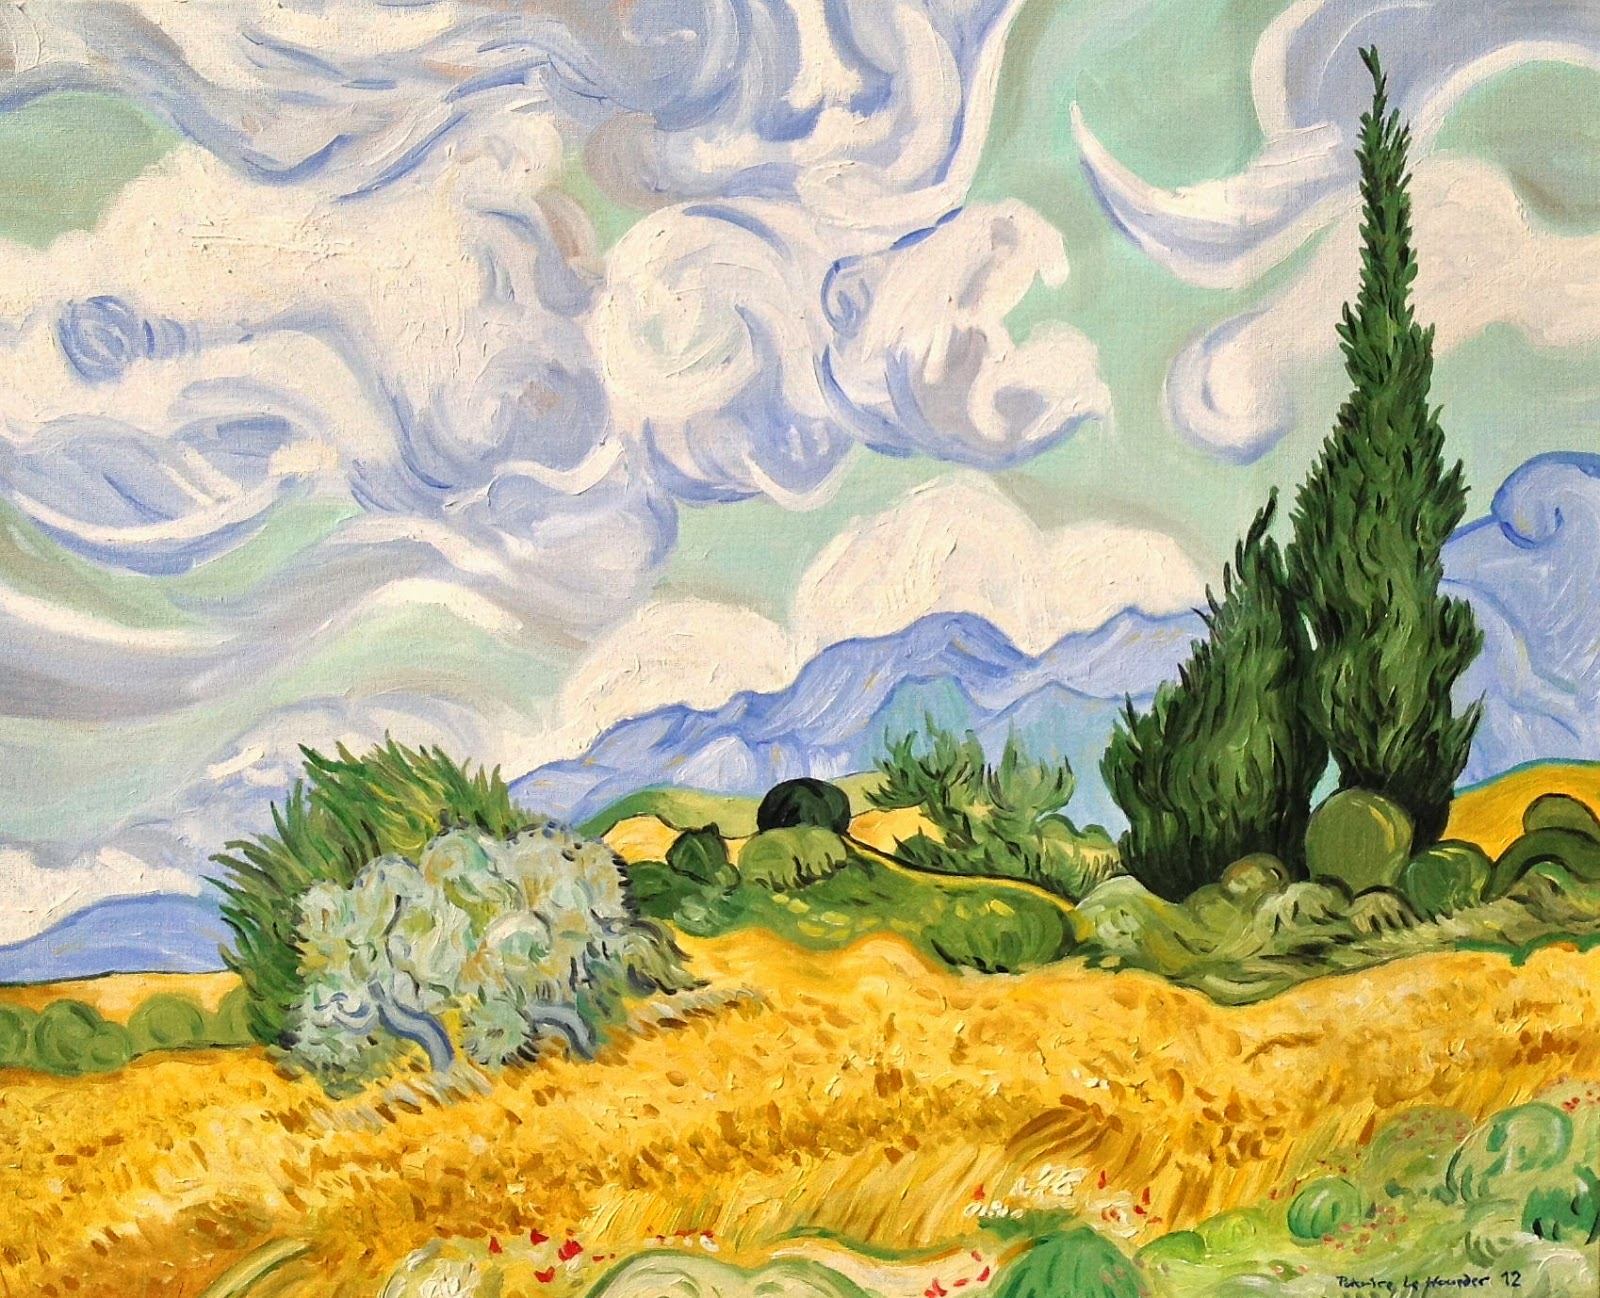
\includegraphics[scale=1.25]{v.jpg}}} % Image background
\begin{tikzpicture}[remember picture,overlay]
%ដាក់ផ្ទាំងពីក្រោយជា pdf
%\node[inner sep=0pt] (background) at (current page.center) {
\includegraphics[width=\paperwidth]{background}};
%ដាក់ផ្ទាំងពីក្រោយជា រូបភាព
\draw (current page.center) node [fill=ocre!70!white,fill opacity=0.6,text opacity=1,inner sep=1cm]{\Huge\centering\bfseries\sffamily\parbox[c][][t]{\paperwidth}{\centering \color{white} \kml ដេរីវេនៃអនុគមន៍\\[15pt] % Book title
{\Large \color{white} \kml ថ្នាក់ទី ១២}\\[20pt] % Subtitle
{ \color{white} \kbk ស៊ុំ សំអុន}}}; % Author name
\end{tikzpicture}
\vfill
\endgroup

%----------------------------------------------------------------------------------------
%	COPYRIGHT PAGE
%----------------------------------------------------------------------------------------

\newpage
~\vfill
\thispagestyle{empty}

%\noindent Copyright \copyright\today\\ % Copyright notice
%
%\noindent \textsc{ Published by Publisher}\\ % Publisher
 
%----------------------------------------------------------------------------------------
%	TABLE OF CONTENTS
%----------------------------------------------------------------------------------------

%\usechapterimagefalse % If you don't want to include a chapter image, use this to toggle images off - it can be enabled later with \usechapterimagetrue

\chapterimage{band1.png} % Table of contents heading image

\pagestyle{empty} % No headers

\tableofcontents % Print the table of contents itself

\cleardoublepage % Forces the first chapter to start on an odd page so it's on the right

%\usepackage{fancyhdr}
\pagestyle{fancy}
\lfoot{\kbk រៀបរៀងដោយ៖ \kbk ស៊ំុ សំអុន}
\cfoot{\kbk \color{magenta}​\thepage}
\rfoot{\kbk ទូរស័ព្ទលេខ៖ \kbk ០៩៦ ៩៤០ ៥៨៤០ }


%----------------------------------------------------------------------------------------
%	PART
%----------------------------------------------------------------------------------------

\part{\kml \color{magenta} ពិជគណិត}

%----------------------------------------------------------------------------------------
%	CHAPTER 1
%----------------------------------------------------------------------------------------

\chapterimage{band1.png} % Chapter heading image

\chapter{ដេរីវេនៃអនុគមន៍}
%\section{\centering ដេរីវេនៃអនុកមន៍}
\section{និយមន័យ}
\begin{definition}
ដេរីវេនៃអនុគមន៍ $y=f(x)$ ត្រង់ $a$ កំណត់ដោយ 
\begin{align}\label{def1}
 f'(a)&=\lim _{x\to a}\dfrac{f(x)-f(a)}{x-a} \;\text{។}
 \end{align}
  \end{definition}
\begin{itemize}
\item អនុគមន៍ $f$ មានដេរីវេលើចន្លោះបើក $(b,c)$ កាលណា $f$ មានដេរីវេលើគ្រប់ចំណុច
 $a\in (b,c)$ ។
\item អនុគមន៍ $f$ មានដេរីវេលើចន្លោះបិទ $[b,c]$ កាលណា $f$ មានដេរីវេលើចន្លោះ $(b,c)$ ហើយ $f$
 មានដេរីវេខាងឆ្វេងត្រង់ $x=b$ និងខាងស្តាំត្រង់ $x=c$ ។ 
 \end{itemize}
\begin{example}
រកដេរីវេនៃអនុគមន៍ $y=f(x)=2x^2+3$ ត្រង់ $2$ ។
\end{example}
\answer
\begin{align*}
f'(2)&=\lim_{x\to 2}\dfrac{f(x)-f(2)}{x-2}\; \text{ដែល } \; f(2)=2(2)^2+3=11\\
f'(2)&=\lim_{x\to 2}\dfrac{2x^2+3x-11}{x-2}\\
&=\lim_{x\to 2}\dfrac{2x^2-8}{x-2}\\
&=\lim_{x\to 2}\dfrac{2(x+2)(x-2)}{x-2}\; ,x\neq 2\\
&=2\times 4=8
\end{align*}
\subsection{ការកំណត់សរសេរ}
តាង $h=x-a\Longrightarrow x=h+a$ បើ $h\longrightarrow 0$ នោះ $x\longrightarrow a$ នោះសមីការ (\ref{def1}) គេបាន
\begin{align}\label{def2}
f'(a)&=\lim_{h\to 0}\dfrac{f(h+a)-f(a)}{h}
\end{align}
\begin{notation}
គេអាចសរសេរដេរីវេដោយ $y' \;, \; f'(x)$ ឬ $\dfrac{dy}{dx}$ ។ 
\end{notation}
\begin{example}
ស្រាយថាបើ $y=x$ នោះ $y'=1$ ។
\solution 
តាមនិយមន័យ 
\begin{align*}
f'(x)&=\lim_{h\to 0}\dfrac{f(h+x)-f(x)}{h} \;\text {ដែល}\; y=f(x)=x ,f(h+x)=h+x\\
&=\lim_{h=\to 0}\dfrac{h+x-x}{h}=\lim_{h\to 0}1=1\\
\therefore \quad \dfrac{dy}{dx}&=1
\end{align*}
\end{example}
\begin{theorem}
បើអនុគមន៍ $f$ មានដេរីវេត្រង់ $x_0$ នោះ $f$ ជាប់ត្រង់ $x_0$ ។
\end{theorem}
\solution 
\begin{align*}
\text{គេនឹងបង្ហាញថា បើ} \; f'(a)&=\lim_{x\to a}\dfrac{f(x)-f(a)}{x-a} \; \text{នោះ}  \;  \lim_{x\to a}f(x)=f(a) \\
\text{គេមាន} \quad \lim_{x\to a}f(x)&=\lim_{x\to a}\left(f(x)-f(a)+f(a) \right)\\
&=\lim_{x\to a}\left(\dfrac{f(x)-f(a)}{x-a}\times (x-a)+f(a) \right)\\
&=\lim_{x\to a}\dfrac{f(x)-f(a)}{x-a}\times \lim_{x\to a}(x-a)+f(a)\\
&=f'(a)\times 0+f(a)\\
&=f(a)
\end{align*}
\begin{notation}
បើអនុគមន៍ $f$ ជាប់ត្រង់ $x_0$ នោះ $f$ អាចមានដេរីវេត្រង់ $x_0$ ឬ គ្មានដេរីវេត្រង់ $x_0$ ។
\end{notation}
\section{ភាពមានដេរីវេ}
\begin{definition}
អនុគមន៍ $f$ មានដេរីវេត្រង់ $x$ លុះត្រាតែ 
\begin{itemize}
\item អនុគមន៍ $f$ ជាប់ត្រង់ $x$ ។
\item ដេរីវេឆ្វេងស្មើដេរីវេស្តាំត្រង់ចំណុច $x$ គឺ $f'_-(x)=f'_+(x)$ ដែល \\
$f'_-(x)=\lim_{h\to 0^-}\dfrac{f(x+h)-f(x)}{h}$ និង $f'_+(x)=\lim_{h\to 0^+}\dfrac{f(x+h)-f(x)}{h}$ ។
\end{itemize}
\end{definition}
\begin{example}
គេឲ្យអនុគមន៍ $f$ កំណត់ដោយ $f(x)=\begin{cases}
\cos x   &$ បើ $x\leq \frac{\pi}{4}\\
a+bx & $ បើ $x> \frac{\pi}{4}
\end{cases}$  \\
កំណត់តម្លៃ $a$ និង $b$ ដើម្បីឲ្យអនុគមន៍ $f$ មានដេរីវេត្រង់ $x=\frac{\pi}{4}$ ។
\end{example}
\solution
\begin{itemize}
\item បើអនុគមន៍ $f$ ជាប់ត្រង់ $x=\frac{\pi}{4}$ នោះ $\lim_{x\to \frac{\pi}{4}^-}f(x)=\lim_{x\to \frac{\pi}{4}^+}f(x)=f\left(\frac{\pi}{4}\right)\\
\lim_{x\to \frac{\pi}{4}^-}\cos x=\lim_{x\to \frac{\pi}{4}^+}(a+bx)=\cos \frac{\pi}{4}\Longleftrightarrow \dfrac{\sqrt{2}}{2}=a+b.\dfrac{\pi}{4}=\dfrac{\sqrt{2}}{2}\Longrightarrow a=\dfrac{\sqrt{2}}{2}-\dfrac{\pi}{4}.b$
\item ដេរីវេឆ្វេង $f'_-(x)$
\begin{align*}
f'_-\left(\frac{\pi}{4}\right)&=\lim_{h\to 0^-}\dfrac{f(\frac{\pi}{4}+h)-f\left(\frac{\pi}{4}\right)}{h}\;, f(x)=\cos x\\
&=\lim_{h\to 0^-}\dfrac{\cos (\frac{\pi}{4}+h)-\cos \frac{\pi}{4}}{h}\\
&=\lim_{h\to 0^-}\dfrac{\cos \frac{\pi}{4}\cos h-\sin \frac{\pi}{4}\sin h-\cos \dfrac{\pi}{4}}{h}\\
&=\lim_{h\to 0^-}\dfrac{-\cos \frac{\pi}{4}(1-\cos h)-\sin \frac{\pi}{4}\sin h}{h}\\
&=\dfrac{\sqrt{2}}{2}\lim_{h\to 0^-}\left(-\dfrac{1-\cos h}{h}-\dfrac{\sin h}{h} \right) \; ,\; \lim_{h\to 0^-}\dfrac{1-\cos h}{h}=0 , \lim_{h\to 0^-}\dfrac{\sin h}{h}=1\\
&=\dfrac{\sqrt{2}}{2}(0-1)=-\dfrac{\sqrt{2}}{2}
\end{align*}
\item ដេរីវេស្តាំ $f'_+(x)$ 
\begin{align*}
f'_+\left(\frac{\pi}{4}\right)&=\lim_{h\to 0^+}\dfrac{f(\frac{\pi}{4}+h)-f\left(\frac{\pi}{4}\right)}{h}\;, f(x)=a+bx\\
&=\lim_{h\to 0^+}\dfrac{a+b(\frac{\pi}{4}+h)-(a+b.\frac{\pi}{4}))}{h}\\
&=\lim_{h\to 0^+}\dfrac{a+b.\frac{\pi}{4}+bh-a-b.\frac{\pi}{4}}{h}\\
&=\lim_{h\to 0^+}\dfrac{bh}{h}=b
\end{align*}
ដោយ $f$ មានដេរីវេត្រង់ $x=\frac{\pi}{4}$ នោះ $f'_-(\frac{\pi}{4})=f'_+(\frac{\pi}{4})\Longleftrightarrow b=-\dfrac{\sqrt{2}}{2}\Longrightarrow a=\dfrac{\sqrt{2}}{2}\left(1+\dfrac{\pi}{4}\right)$
\end{itemize}
 \section{លក្ខណះនៃដេរីវេ}
 \begin{property}
 ចំពោះ $u,v$ ជាអនុគមន៍នៃ $x$ និង $k$ ជាចំនួនថេ នោះគេបាន៖
 \begin{multicols}{3}
 \begin{enumerate}
 \item $(ku)'=ku'$
 \item $(u+ v)'=u'+ v$
 \item $(u-v)'=u'-v'$
 \item $(uv)'=u'v+v'u$
 \item $\left(\dfrac{u}{v}\right)'=\dfrac{u'v-v'u}{v^2}$
 \item $\left(\dfrac{1}{v}\right)'=-\dfrac{v'}{v^2}$
 \end{enumerate}
 \end{multicols}
 \end{property}
 \solution 
\begin{enumerate} 
\item តាង $f(x)=k.u(x)$  ដែល $u=u(x)$ និង $k$ ជាចំនួនថេ តាមនិយមន័យ
 \begin{align*}
  f'(x)&=\lim_{h\to 0}\dfrac{f(x+h)-f(x)}{h}\\
 &=\lim_{h\to 0}\dfrac{ku(x+h)-k.u(x) }{h}\\
 &=k.\lim_{h\to 0}\dfrac{u(x+h)-u(x)}{h}\\
 &=k.u'(x)\\
 \therefore \quad (k.u)'&=k.u'
 \end{align*}
\item តាង $f(x)=u(x)+ v(x)$  ដែល $u=u(x)$ និង $v=v(x)$ តាមនិយមន័យ
 \begin{align*}
  f'(x)&=\lim_{h\to 0}\dfrac{f(x+h)-f(x)}{h}\\
 &=\lim_{h\to 0}\dfrac{u(x+h)+ v(x+h)-(u(x)+ v(x)) }{h}\\
 &=\lim_{h\to 0}\dfrac{u(x+h)-u(x)}{h}+\lim_{h\to 0}\dfrac{v(x+h)-v(x)}{h}\\
 &=u'(x)+v'(x)\\
 \therefore \quad (u+v)'&=u'+v'
 \end{align*}
 \item ស្រាយដូចទី២
 \item តាង $f(x)=uv$ ដែល $u=u(x)$ និង $v=v(x)$ តាមនិយមន័យគេបាន
 \begin{align*}
 f'(x)&=\lim_{h\to 0}\dfrac{f(x+h)-f(x)}{h}\\
 &=\lim_{h\to 0}\dfrac{u(x+h).v(x+h)-u(x).v(x)}{h}\\
 &=\lim_{h\to 0}\dfrac{u(x+h).v(x+h)-u(x).v(x+h)+u(x).v(x+h)+u(x).v(x)}{h}\\
 &=\lim_{h\to 0}\left[\dfrac{u(x+h).v(x+h)-u(x).v(x+h)}{h}+\dfrac{u(x).v(x+h)+u(x).v(x)}{h}\right]\\
  &=\lim_{h\to 0}\left[v(x+h).\dfrac{u(x+h)-u(x)}{h}+u(x).\dfrac{v(x+h)+v(x)}{h}\right]\\
  &=v(x).\dfrac{d}{dx}(u(x))+u(x).\dfrac{d}{dx}(v(x))
 % \therefore \quad (uv)'&=u'v+v'u 
 \end{align*}
 \begin{align}\label{eq5}
 \therefore\quad (uv)'=u'v+v'u
 \end{align}
 \item យក $u=u(x)$ និង $v=v(x)$ តាង $f(x)=\dfrac{u}{v}\Leftrightarrow f(x).v=u$ ធ្វើដេរីវេអង្គទាំងពីរធៀបនឹង $x$ \\
 នោះគេបាន $[f(x).v]'=u'$ ប្រើតាមសមីការ (\ref{eq5}) គេបាន
\begin{align*}
f'(x).v+v'f(x)&=u' ,\; f(x)=\dfrac{u}{v}\\
f'(x).v+v'. \dfrac{u}{v}&=u'\\
\dfrac{f'(x).v^2}{v}+\dfrac{v'u}{v}&=u'\\
f'(x).v^2+v'u&=u'v\\
  f'(x)&=\dfrac{u'v-v'u}{v^2}
\end{align*}
\begin{align}\label{eq6}
\therefore\quad\left(\dfrac{u}{v}\right)'=\dfrac{u'v-v'u}{v^2}
\end{align}
\item យក $v=v(x)$ តាង $f(x)=\dfrac{1}{v}$ ប្រើសមីការ (\ref{eq6}) គេបាន 
\begin{align*}
f'(x)&=\dfrac{(1)'.v-v'.(1)}{v^2}\\
&=\dfrac{0-v'}{v^2}\\
&=-\dfrac{v'}{v^2}\\
\therefore \quad\left( \dfrac{1}{v}\right)'&=-\dfrac{v'}{v^2}
\end{align*}

 \end{enumerate}
 \section{ដេរីវេនៃអនុគមន៍បណ្តាក់}
 \begin{general}
 បើ $y=f(u)$ និង $u=g(x)$ នោះ $\dfrac{d}{dx}(f \circ g)=\dfrac{dy}{dx}=\dfrac{dy}{du}\times \dfrac{du}{dx}$  ។ 
 \end{general}
 \solution តាង $F(x)=f\circ g=f(g(x))$  តាមនិយមន័យភាពមានដេរីវេត្រង់ $x=a$ នោះគេបាន 
 \begin{align*}
 F'(a)&=\lim_{x\to a}\dfrac{F(x)-F(a)}{x-a}\\
 &=\lim _{x\to a}\dfrac{f(g(x))-f(g(a))}{x-a}\\
 &=\lim_{x\to a}\left( \dfrac{f(g(x))-f(g(a))}{g(x)-g(a)} \times \dfrac{g(x)-g(a)}{x-a}\right)\\
 &=f'(g(a))\times g'(a)\quad,u=g(a),y=f(a)\\
 \therefore \quad \dfrac{d}{dx}(f\circ g)=\dfrac{dy}{dx}&=\dfrac{dy}{du}\times \dfrac{du}{dx}
 \end{align*}
 
\begin{general}
បើ $y=c$ ដែល $c$ ជាចំនួនថេរ នោះ $y'=0$ ។  
\end{general}
\solution 
គេមាន $y=f(x_0)=c$ នោះ $f(x_0+h)=c \;, c\in \R$
តាមនិយមន័យគេបាន 
\begin{align*}
f'(x)&=\lim_{h\to 0}\dfrac{f(x+h)-f(x)}{h}\\
&=\lim_{h\to 0}\dfrac{c-c}{h}\\
&=\lim_{h\to 0}\dfrac{0}{h}\\
\therefore \quad \dfrac{d}{dx}(c)&=0
\end{align*}

\begin{example}
គណនា $y'$ ដែល $y=\left(\ln x .\log_a (\sqrt{3}) \right)$ ។
\end{example}
\answer 
គេមាន $y=\left(\ln x .\log_a (\sqrt{3}) \right)\Rightarrow y'=\left(\ln x .\log_a (\sqrt{3}) \right)'=0$
\begin{example}
ស្រាយបញ្ជាក់ថា បើ $y=x^n$ នោះ $y'=nx^{n-1}$ ។
\end{example}
\solution
គេមាន $f(x)=x^n$ នាំឲ្យ $f(x+h)=(x+h)^n$ តាមនិយមន័យ
\begin{align*}
y'=f'(x)&=\lim_{h\to 0}\dfrac{f(x+h)-f(x)}{h}\\
&=\lim_{h\to 0}\dfrac{(x+h)^n-x^n}{h}\\
&=\lim_{h\to 0}\dfrac{(x+h-x)(x^{n-1}+x^{n-2}.x+...+x.x^{n-2}x+x^{n-1})}{h}\\
&=\lim_{h\to 0}(x^{n-1}+x^{n-1}+...+x^{n-1}+x^{n+1})\\
&=x^{n-1}(\underbrace{1+1+...+1+1}_{n\; \text{តួរលេខ 1}})\\
&=n.x^{n-1}\\
\therefore \quad \dfrac{d}{dx}(x^n)&=n.x^{n-1}
\end{align*}
%---------------------------- example-----------------------------
\begin{example}
គណនា $f'(x)$ 
\begin{multicols}{3}
\begin{enumerate}
\item $f(x)=x^3$
\item $f(x)=\sqrt{x}$
\item $f(x)=\sqrt[3]{x^2}$
\end{enumerate}
\end{multicols}
\end{example}
\answer 
\begin{enumerate}
\item $f(x)=x^3 \Rightarrow f'(x)=(x^3)'=3 x^{3-1}=3x^2$
\item $f(x)=\sqrt{x} \Rightarrow f'(x)=(\sqrt{x})'=(x^{\frac{1}{2}})'=\dfrac{1}{2}x^{\frac{1}{2}-1}=\dfrac{1}{2}x^{-\frac{1}{2}}=\dfrac{1}{2\sqrt{x}}$
\item $f(x)=\sqrt[3]{x^2}\Rightarrow f'(x)=(\sqrt[3]{x^2})'=(x^{\frac{2}{3}})'=\dfrac{2}{3}x^{\frac{2}{3}-1}=\dfrac{2}{3}x^{-\frac{1}{3}}=\dfrac{2}{3\sqrt[3]{x}}$
\end{enumerate}
%-------------------------------- general --------------------------
\begin{general}
បើ $y=u^n$ ដែល $u$ ជាអនុគមន៍នៃ $x$ នោះ $y'=n u' u^{n-1}$  ។  
\end{general}
\solution
គេមាន $y=u^n$ គេបាន $y'=\dfrac{dy}{dx}=\dfrac{dy}{du}\times \dfrac{du}{dx}=\dfrac{d}{du}(u^n)\times u'=nu'u^{n-1}$ 
\begin{example}
គណនា $y'$ 
\begin{multicols}{2}
\begin{enumerate}
\item $y=(2x+\ln 2)^4$
\item $y=\sqrt{u}$ ដែល $u$ ជាអនុគមន៍នៃ $x$ ។
\end{enumerate}
\end{multicols}
\end{example}
\answer
\begin{enumerate}

\item $y=(2x+\ln 2)^4\Longrightarrow y'=4(2x+\ln 2)'(2x+\ln 2)^{4-1}=4(2+0)(2x+\ln 2)^3$
\begin{center}
$\therefore \quad y'=8(2x+\ln 2)^3$
\end{center}
\item $y=\sqrt{u}=u^{\frac{1}{x}} \Longrightarrow y'=(u^{\frac{1}{2}})'=\dfrac{1}{2}u'u^{\frac{1}{2}-1}=\dfrac{1}{2}u'u^{-\frac{1}{2}}=\dfrac{u'}{2\sqrt{u}}$ ។ 
\end{enumerate}
\section{ដេរីវេនៃអនុគមន៍ត្រីកោណមាត្រ}
\begin{property}
ដេរីវេអនុគមន៍ត្រីកោណមាត្រ
\begin{enumerate}
%\begin{multicols}{2}
\item បើ $y=\sin x$ នោះ $y'=\cos x$ 
\item បើ $y=\cos x$ នោះ $y'=-\sin x$
%\end{multicols}
\item បើ $y=\tan x$ នោះ $y'=\dfrac{1}{\cos^2 x}=1+\tan^2 x$
\item បើ $y=\cot x$ នោះ $y'=-\dfrac{1}{\sin^2 x}=-(1+\cot^2 x)$
\end{enumerate}
\end{property}
%------------------------------------solution-----------------------
\solution
%-------------------------------------------1--------------------------------------------
\begin{enumerate}
\item គេមាន $y=f(x)=\sin x$ នោះ $f(x+h)=\sin (x+h)$ តាមនិយមន័យ 
\begin{align*}
y'=f'(x)&=\lim_{h\to 0}\dfrac{f(x+h)-f(x)}{h}\\
&=\lim_{h\to 0}\dfrac{\sin (x+h)-\sin x}{h}\\
&=\lim_{h\to 0}\dfrac{\sin x\cos h+\sin h.\cos x -\sin x}{h}\\
&=\lim_{h\to 0}\left(\cos x.\dfrac{\sin h}{h}-\sin x.\dfrac{1-\cos h}{h}  \right)\\
&=\cos x \quad , \lim_{h\to 0}\dfrac{\sin h}{h}=1, \lim_{h\to 0}\dfrac{1-\cos h}{h}=0\\
\therefore \quad \dfrac{d}{dx}(\sin x)&=\cos x
\end{align*} 
%--------------------------------2-----------------------------
\item គេមាន $y=f(x)=\cos x$ នោះ $f(x+h)=\cos (x+h)$ តាមនិយមន័យ
\begin{align*}
y'=f'(x)&=\lim_{h\to 0}\dfrac{f(x+h)-f(x)}{h}\\
&=\lim_{h\to 0}\dfrac{\cos (x+h)-\cos x}{h}\\
&=\lim_{h\to 0}\dfrac{\cos x.\cos h-\sin x .\sin h-\cos x}{h}\\
&=\lim_{h\to 0}\left(-\dfrac{\sin h}{h}.\sin x-\cos x. \dfrac{1-\cos h}{h} \right)\\
&=-\sin x \quad , \lim_{h\to 0}\dfrac{1-\cos h}{h}=0,\lim_{h\to 0}\dfrac{\sin h}{h}=1\\
\therefore\quad \dfrac{d}{dx}(\cos x)&=-\sin x
\end{align*}
%----------------------------------------3----------------------
\item តាង $y=\tan x=\dfrac{\sin x}{\cos x}$ តាមសមីការ (\ref{eq6}) គេបាន 
\begin{align*}
y'=\left(\dfrac{\sin x}{\cos x} \right)'&=\dfrac{(\sin x)'\cos x-(\cos x)'.\sin x}{(\cos x)^2}\\
&=\dfrac{\cos x.\cos x-(-\sin x).\sin x}{\cos^2 x}\\
&=\dfrac{\cos^2 x+\sin^2 x}{\cos^2 x}\\
&=1+\tan^2 x\\
&=\dfrac{1}{\cos^2 x} ,\; \sin^2 x+\cos^2 x=1\\
\therefore \quad (\tan x)'&=\dfrac{1}{\cos^2}=1+\tan^2 x
\end{align*}
%--------------------------------------------4-------------------
\item តាង $y=\cot x=\dfrac{\cos x}{\sin x}$ តាមសមីការ (\ref{eq6}) គេបាន
\begin{align*}
y'=\left(\dfrac{\cos x}{\sin x} \right)'&=\dfrac{(\cos x)'.\sin x-(\sin x)'.\cos x}{(\sin^2x)^2}\\
&=\dfrac{-\sin x. \sin x-\cos x.\cos x}{\sin^2 x}\\
&=\dfrac{-\sin^2 x-\cos^2 x}{\sin^2 x}\\
&=-\dfrac{\sin^2 x+\cos^2 x}{\sin^2 x} \;, \sin^2 x+\cos^2 x=1\\
\therefore \quad (\cot x)'&=-\dfrac{1}{\sin^2 x}=-(1+\cot^2x) 
\end{align*}
\end{enumerate}
%--------------------------------general ------------------------
\begin{general}
បើ $u$ ជាអនុគមន៍នៃ $x$ គេបាន 
\begin{enumerate}
%\begin{multicols}{2}
\item បើ $y=\sin u$ នោះ $y'=u'\cos u$ 
\item បើ $y=\cos u$ នោះ $y'=-u'\sin u$  
%\end{multicols}
\item បើ $y=\tan u$ នោះ $y'=\dfrac{u'}{\cos^2 u}=u(1+\tan^2 u)$
\item បើ $y=\cot u$ នោះ $y'=-\dfrac{u'}{\sin^2 u}=-u'(1+\cot^2 u)$
\end{enumerate}

\end{general}
\solution 
\begin{enumerate}

%---------------------------------------1----------------------
\item បើ $u$ ជាអនុគមន៍នៃ $x$ នោះ $y=\sin u$ គេបាន 
\begin{align*}
\dfrac{dy}{dx}=\dfrac{dy}{du}\times \dfrac{du}{dx}&=\dfrac{d}{du}(\sin u)\times \dfrac{du}{dx}=\cos u \times u'=u'\cos u\\
\therefore \quad \dfrac{d}{dx}(\sin u)&=u'\cos u
\end{align*}
%------------------------------------2-----------------------
\item បើ $u$ ជាអនុគមន៍នៃ $x$ នោះ $y=\cos u$ គេបាន 
\begin{align*}
\dfrac{dy}{dx}=\dfrac{dy}{du}\times \dfrac{du}{dx}&=\dfrac{d}{du}(\cos u)\times \dfrac{du}{dx}=-\sin u \times u'=-u'\sin u\\
\therefore \quad \dfrac{d}{dx}(\cos u)&=-u'\sin u
\end{align*}
%-------------------------------------5---------------------------------
\item បើ $u$ ជាអនុគមន៍នៃ $x$ នោះ $y=\tan u$ គេបាន 
\begin{align*}
\dfrac{dy}{dx}=\dfrac{dy}{du}\times \dfrac{du}{dx}&=\dfrac{d}{du}(\tan u)\times \dfrac{du}{dx}=\dfrac{1}{\cos^2 u} \times u'=(1+\tan^2 u)\times u'\\
\therefore \quad (\tan u)'&=\dfrac{u'}{\cos^2 u}=u'(1+\tan^2 u)
\end{align*}
%--------------------------------------------6--------------------------------------
\item បើ $u$ ជាអនុគមន៍នៃ $x$ នោះ $y=\cot u$ គេបាន 
\begin{align*}
\dfrac{dy}{dx}=\dfrac{dy}{du}\times \dfrac{du}{dx}&=\dfrac{d}{du}(\cot u)\times \dfrac{du}{dx}=-\dfrac{1}{\sin^2 u} \times u'=-(1+\cot^2 u)\times u'\\
\therefore \quad (\cot u)'&=-\dfrac{u'}{\sin ^2 u}=-u'(1+\cot^2 u)
\end{align*}
\end{enumerate}
%--------------------------------------------- example----------------------------
\begin{example}
គណនាដេរីវេនៃអនុគមន៍ខាងក្រោម៖
\begin{multicols}{2}
\begin{enumerate}
\item $y=\sin (2x+1)$
\item $y=\cos (2x+1)$
\item $y=\tan (2x+1)$
\item $y=\cot (2x+1)$ ។
\end{enumerate}
\end{multicols}
\end{example}
\answer 
\begin{enumerate}
\item $y=\sin (2x+1) \Rightarrow y'=(2x+1)'\cos (2x+1)=2\cos (2x+1)$
\item $y=\cos (2x+1)\Rightarrow y'=-(2x+1)'\sin (2x+1)=-2\sin (2x+1)$
\item $y=\tan (2x+1)\Rightarrow y'=\dfrac{(2x+1)'}{\cos^2 (2x+1)}=\dfrac{2}{\cos^2 (2x+1)}=2[1+\tan^2(2x+1)]$
\item $y=\cot (2x+1)\Rightarrow y'=-\dfrac{(2x+1)'}{\sin ^2 (2x+1)}=-\dfrac{2}{\sin^2 (2x+1)}=-2[1+\cot^2 (2x+1)]$ ។
\end{enumerate}
\section{ដេរីវេអនុគមន៍អិចស្ប៉ូណង់ស្យែល}
ស្រាយថាបើ $y=a^x$ នោះ $y'=a^x .\ln a$
\solution
គេមាន $y=a^x$ តាមនិយមន័យ គេបាន
\begin{align*}
y'=f'(x)&=\lim_{h\to 0}\dfrac{f(x+h)-f(x)}{h}\\
&=\lim_{h\to 0}\dfrac{a^{x+h}-a^{x}}{h}\\
&=\lim_{h\to 0}\dfrac{a^{x}(a^h-1)}{h}\\
&=a^{x}\lim_{h\to 0}\dfrac{a^h-1}{h}\;\text{ដោយ}\; \lim_{x\to 0}\dfrac{a^x-1}{x}=\ln a\\
%&=a^{x}.\ln a\\
\therefore \quad (a^x)'&=a^x. \ln a
\end{align*}
\begin{general}
បើ $u$ ជាអនុគមន៍នៃ $x$ នោះ $(a^u)'=u'a^u.\ln a$ ។ 
\end{general}
\solution 
បើ $u$ ជាអនុគមន៍នៃ $x$ នោះ  គេបាន 
\begin{align*}
\dfrac{dy}{dx}=\dfrac{dy}{du}\times \dfrac{du}{dx}&=\dfrac{d}{du}(a^u)\times \dfrac{du}{dx}=a^u.\ln a \times u'\\
\therefore \quad (a^u)'&=u'.a^u .\ln a)
\end{align*}
%--------------------example-------
\begin{example}
គណនា $y'$ ចំពោះ $u$ ជាអនុគមន៍នៃ $x$ នៃអនុគមន៍ខាងក្រោម៖
\begin{multicols}{3}
\begin{enumerate}
\item $y=e^x$  
\item $y=a^{x^2-1}$
\item $y=e^u$ 
\end{enumerate}
\end{multicols}
\end{example}
\answer
\begin{enumerate}
 \item  $y=e^x$ នោះ $y'=(e^x)'=e^x.\ln e=e^x\;,\ln e=1$ 
 \item $y=a^{x^2-1}$ នោះ $y'=(x^{x^2-1})'a^{x^2-1}\ln a=2x.a^{x^2-1}\ln a$
\item $y=e^u$ នោះ $y'=(e^u)'=u'e^u.\ln e=u'e^u\;,\;\ln e=1$
\end{enumerate}
\section{ដេរីវេនៃអនុគមន៍កោការីត}
ស្រាយបញ្ជាក់ថា បើ $y=\log _a x \;, a>0,a\neq 1$ នោះ $y'=\dfrac{1}{x\ln a}$ ។
\solution 
គេមាន $y=\log_a x$ តាមនិយមន័យ គេបាន
\begin{align*}
y'=f'(x)&=\lim_{h\to 0}\dfrac{f(x+h)-f(x)}{h}\\
&=\lim_{h\to 0}\dfrac{\log_a (x+h)-\log_a (x)}{h}\\
&=\lim_{h\to 0}\dfrac{1}{h}\log_a \left(\dfrac{x+h}{x} \right)\\
&=\lim_{h\to 0}\log_a \left(1+\dfrac{h}{x} \right)^\dfrac{1}{h}\\
&=\log_a \left(\lim_{h\to 0}\left(1+\dfrac{1}{\frac{x}{h}}\right)^{\dfrac{x}{h}}\right)^\dfrac{1}{x}\; \text{ដោយ }\lim_{x\to 0}(1+\dfrac{1}{x})^x=e\\
&=\log_a e^{\dfrac{1}{x}}=\dfrac{1}{x}\dfrac{\ln e}{\ln a}\\
\therefore \quad (\log_a x)'&=\dfrac{1}{x\ln a}\;, a>0,a\neq 1
\end{align*}

\begin{general}
បើ $u$ ជាអនុគមន៍នៃ $x$ នោះ $(\log_a u)'=\dfrac{u'}{u\ln a}\;, a>0,a\neq 1$ ។ 
\end{general}
\solution 
បើ $u$ ជាអនុគមន៍នៃ $x$ នោះ  គេបាន 
\begin{align*}
\dfrac{dy}{dx}=\dfrac{dy}{du}\times \dfrac{du}{dx}&=\dfrac{d}{du}(\log_a u)\times \dfrac{du}{dx}=\dfrac{1}{u\ln a}\times u'\\
\therefore \quad (\log_a u)'&=\dfrac{u'}{u\ln a} \;, a>0,a\neq 1
\end{align*}

\section{ដេរីវេនៃអនុគមន៍លោការីតនេពែ}
ស្រាយបញ្ជាក់ថា បើ $y=\ln x$ នោះ $y'=\dfrac{1}{x}$ ។
\solution 
គេមាន $y=\ln x$ តាមនិយមន័យ គេបាន
\begin{align*}
y'=f'(x)&=\lim_{h\to 0}\dfrac{f(x+h)-f(x)}{h}\\
&=\lim_{h\to 0}\dfrac{\ln (x+h)-\ln (x)}{h}\\
&=\lim_{h\to 0}\dfrac{\ln \left(\dfrac{x+h}{x} \right)}{h}\\
&=\lim_{h\to 0}\dfrac{1}{h}\ln \left(1+\dfrac{h}{x} \right)\\
&=\lim_{h\to 0}\ln \left(1+\dfrac{h}{x}\right)^{\dfrac{1}{h}}\\
&=\ln \left[\lim_{h\to 0}\left(1+\dfrac{1}{\frac{x}{h}} \right)^{\frac{x}{h}\times \frac{1}{x}}  \right]\;, \lim_{h\to 0}\left(1+\dfrac{1}{\frac{x}{h}} \right)^{\frac{x}{h}}=e\\
&=\ln e^{\dfrac{1}{x}},\ln e=1\\
\therefore \quad (\ln x)'&=\dfrac{1}{x} 
\end{align*}
%----------------------------------------- example ----------------------------
\begin{example}
រក $f'(x)$ នៃអនុគមន៍ខាងក្រោម៖
\begin{multicols}{2}
\begin{enumerate}
\item $f(x)=x^2.\log_a x, a>0,a\neq 1$
\item $f(x)=\sin (2x)+\log_2 (x^2+1)$
\item $f(x)=\dfrac{e^{2x}+\log_3 x}{x^2}$
\item $f(x)=\log (x^2 \sqrt{x^3-1})$
\item $f(x)=(\sin x)^{\log x}$
\item $f(x)=(\log _a x)^{\ln (2x)},a>0,a\neq 1$
\end{enumerate}
\end{multicols}
\end{example}

%----------------------------------- solution -----------------------
\solution 
\begin{enumerate}
\item $f(x)=x^2.\log_a x, a>0,a\neq 1\Longrightarrow f'(x)=(x^2)'\log_a x+\left(\log_a x \right)'x^2$
\begin{align*}
&=2x\log_a x+\dfrac{1}{x\ln a}x^2\\
\therefore \quad f'(x)&=2x\log _a x+\dfrac{x}{\ln a} , a>0,a\neq 1
\end{align*}
\item $f(x)=\sin (2x)+\log_2 (x^2+1)\Longrightarrow f'(x)=-(2x)'\cos (2x)+\dfrac{(x^2+1)'}{(x^2+1)\ln 2}$
\begin{center}
$\therefore \quad f'(x)=-2\cos(2x)+\dfrac{2x}{(x^2+1)\ln 2}$
\end{center}
\item $f(x)=\dfrac{e^{2x}+\log_3 x}{x^2}\Longrightarrow f'(x)=\dfrac{(e^{2x}+\log_3 x)'x^2-(x^2)'(e^{2x}+\log_3 x)}{x^4}$
\begin{align*}
&=\dfrac{(2e^{2x}+\dfrac{1}{x\ln 3})x^2-2x(e^{2x}+\log_3 x)}{x^4}\\
&=\dfrac{2xe^{2x}+\dfrac{1}{\ln 3}-2e^{2x}-2\log_3 x}{x^3}\\
\therefore \quad f'(x)&=\dfrac{2e^{2x}(x-1)+\dfrac{1}{\ln 3}-\log_3x^2}{x^3}
\end{align*}
\item $f(x)=\log (x^2 \sqrt{x^3-1})=\log x^2 +\log (x^3-1)^{\frac{1}{2}}=2\log x+\dfrac{1}{2}\log (x^3-1)\\
\therefore \quad f'(x)=\dfrac{2}{x\ln 10}+\dfrac{(x^3-1)'}{2(x^3-1)\ln 10}=\dfrac{2}{x\ln 10}+\dfrac{3x^2}{2(x^3-1)\ln 10} $
\item $f(x)=(\sin x)^{\log x}\Longleftrightarrow \ln f(x)=\ln (\sin x)^{\log x}$
\begin{align*}
\left(\ln f(x) \right)'&=(\log x. \ln (\sin x))'\\
\dfrac{f'(x)}{f(x)}&=(\log x)'\ln (\sin x)+(\ln (\sin x))'\log x\\
f'(x)&=f(x)\left(\dfrac{1}{x\ln 10}\ln (\sin x)+\dfrac{(\sin x)' }{\sin x}.\log x \right)\\
\therefore \quad f'(x)&=(\sin x)^{\log x}\left(\dfrac{\ln (\sin x)}{x\ln 10} +\cot x.\log x\right)
\end{align*}
\item $f(x)=(\log _a x)^{\ln (2x)},a>0,a\neq 1\Longleftrightarrow \ln f(x)=\ln (\log_a x)^{\ln (2x)}$
\begin{align*}
\left(\ln f(x) \right)'&=\left(\ln (2x).\ln (\log_a x) \right)'\\
\dfrac{f'(x)}{f(x)}&=(\ln (2x))'\ln (\log_a x)+(\ln (\log _a x))' \ln (2x)\\
f'(x)&=f(x)\left(\dfrac{(2x)'}{2x}\ln (\log_a x)+\dfrac{(\log _a x)'}{\log_a x}\ln (2x) \right)\\
\therefore \quad f'(x)&=(\log _a x)^{\ln (2x)}\left(\dfrac{\ln (\log_a x)}{x}+\dfrac{\ln (2x)}{x\ln a \log_a x} \right) ,a>0,a\neq 1
\end{align*}
\end{enumerate}


\begin{general}
បើ $u$ ជាអនុគមន៍នៃ $x$ នោះ $(\ln u)'=\dfrac{u'}{u}$ ។ 
\end{general}
\solution 
បើ $u$ ជាអនុគមន៍នៃ $x$ នោះ  គេបាន 
\begin{align*}
\dfrac{dy}{dx}=\dfrac{dy}{du}\times \dfrac{du}{dx}&=\dfrac{d}{du}(\ln u)\times \dfrac{du}{dx}=\dfrac{1}{u}\times u'\\
\therefore \quad (\ln u)'&=\dfrac{u'}{u}
\end{align*}
%----------------------------------------- example ----------------------------
\begin{example}
រក $f'(x)$ នៃអនុគមន៍ខាងក្រោម៖
\begin{multicols}{2}
\begin{enumerate}
\item $f(x)=x.\ln x$
\item $f(x)=x^2+\ln (x^2+1)$
\item $f(x)=\dfrac{e^x+\ln x}{x^2}$
\item $f(x)=\ln (x^2 \sqrt{x^3-1})$
\item $f(x)=x^x$
\item $f(x)=(\sin x)^{\cos x}$
\end{enumerate}
\end{multicols}
\end{example}

%----------------------------------- solution -----------------------
\solution 
\begin{enumerate}
\item $f(x)=x.\ln x\Longrightarrow f'(x)=x'\ln x+(\ln x)' x=\ln x+\dfrac{1}{x}.x=\ln x+1$
\item $f(x)=x^2+\ln (x^2+1)\Longrightarrow f'(x)=(x^2)'+\dfrac{(x^2+1)'}{x^2+1}=2x+\dfrac{2x}{x^2+1}$
\item $f(x)=\dfrac{e^x+\ln x}{x^2}\Longrightarrow f'(x)=\dfrac{(e^x+\ln x)'x^2-(x^2)'(e^x+\ln x)}{(x^2)^2}$
\begin{align*}
&=\dfrac{\left(e^x+\dfrac{1}{x}\right)x^2-2x(e^x+\ln x)}{x^4}\\
\therefore \quad f'(x)&=\dfrac{xe^x+1-2e^x-2\ln x}{x^3}
\end{align*}
\item $f(x)=\ln (x^2 \sqrt{x^3-1})=\ln x^2 +\ln \sqrt{x^3-1}=2\ln x+ \ln (x^3-1)^{\frac{1}{2}}$
\begin{align*}
f'(x)&=2(\ln x)'+\dfrac{1}{2}[\ln (x^3-1)]'\\
&=2.\dfrac{1}{x}+\dfrac{1}{2}.\dfrac{(x^3-1)'}{x^3-1}\\
\therefore \quad f'(x)&=\dfrac{2}{x}+\dfrac{3}{2}.\dfrac{x^2}{x^3-1}
\end{align*}
\item $f(x)=x^x \Longleftrightarrow \ln f(x)=\ln x^x=x\ln x $
\begin{align*}
\left(\ln f(x)\right)'&=(x\ln x)'\\
\dfrac{f'(x)}{f(x)}&=x'\ln x+(\ln x)'x\\
f'(x)&=f(x)(\ln x+\dfrac{1}{x}.x)\\
\therefore \quad f'(x)&=x^x(\ln x+1)
\end{align*}
\item $f(x)=(\sin x)^{\cos x}\Longleftrightarrow \ln f(x)=\ln (\sin x)^{\cos x}$
\begin{align*}
\left(\ln f(x) \right)'&= (\cos x\ln \sin x)'\\
\dfrac{f'(x)}{f(x)}&=(\cos x)'\ln \sin x+(\ln \sin x)'\cos x\\
f'(x)&=f(x)\left(-\sin x\ln sin x+\dfrac{(\sin x)'}{\sin x}.\cos x \right)\\
\therefore \quad f'(x)&=(\sin x)^{\cos x} \left( \cos x\cot x-\sin x\ln \sin x\right)
\end{align*}
\end{enumerate}
\section{ដេរីវេនៃអនុគមន៍ Arc Sine និង Arc  Tangent}
\begin{center}
$y=\arcsin x\Longleftrightarrow x=\sin y$ និង $-\frac{\pi}{2}\leq y \leq \frac{\pi}{2},$\\
$y=\arctan x \Longleftrightarrow x=\tan y$ និង $-\frac{\pi}{2}\leq y \leq \frac{\pi}{2},$
\end{center}
\begin{example}
ស្រាយថា បើ $y=\arcsin x $ នោះ $ y'=\dfrac{1}{\sqrt{1-x^2}}$ ។
\end{example}
\solution
\begin{align*}
\text{បើ}\; y=\arcsin x\; \text{នោះ} \;x&=\sin y \; \text{ធ្វើដេរីវេអង្គសងខាងធៀបនឹង\; $x$\; គេបាន}\\
(x)'&=(\sin y)'\Longleftrightarrow 1=y' \cos y\\
y'&=\dfrac{1}{\cos y} \;\text{ដោយ} \;\sin^2 y+\cos^2 y=1\\
\Longrightarrow \cos y&=\pm\sqrt{1-\sin^2 x}\\
\text{ដោយ}\; -\frac{\pi}{2}\leq y\leq \frac{\pi}{2}&\Longrightarrow\cos y\geq 0 \Longrightarrow \cos y=\sqrt{1-x^2}\\ 
\therefore \quad (\arcsin x)'&=\dfrac{1}{\sqrt{1-x^2}}\\
\end{align*}
\begin{example}
ស្រាយថា បើ $y=\arctan x$ នោះ $y'=\dfrac{1}{1+x^2}$  ។
\end{example}
\solution 
\begin{align*}
\text{បើ} \;y=\arctan x \;\text{នោះ}\' x&=\tan y\; \text{ធ្វើដេរីវេអង្គសងខាងធៀបនឹង\; $x$\; គេបាន}\\
(x)'&=(\sin y)'\Longleftrightarrow 1=y'(1+\tan^2 y )\\
y'&=\dfrac{1}{1+\tan^2 y} \\
\therefore \quad (\arctan x)'&=\dfrac{1}{1+x^2}
\end{align*}
\begin{general}
បើ $u$ ជាអនុគមន៍នៃ $x$ នោះ $(\arcsin u)'=\dfrac{u'}{\sqrt{1-x^2}}$
\end{general}
\solution 
បើ $u$ ជាអនុគមន៍នៃ $x$ នោះ  គេបាន 
\begin{align*}
\dfrac{dy}{dx}=\dfrac{dy}{du}\times \dfrac{du}{dx}&=\dfrac{d}{du}(\arcsin u)\times \dfrac{du}{dx}=\dfrac{1}{\sqrt{1-u^2}}\times u'\\
\therefore \quad (\arcsin u)'&=\dfrac{u'}{\sqrt{1-u^2}}
\end{align*}
\begin{general}
បើ $u$ ជាអនុគមន៍នៃ $x$ នោះ $(\arctan u)'=\dfrac{u'}{1+u^2}$
\end{general}
\solution 
បើ $u$ ជាអនុគមន៍នៃ $x$ នោះ  គេបាន 
\begin{align*}
\dfrac{dy}{dx}=\dfrac{dy}{du}\times \dfrac{du}{dx}&=\dfrac{d}{du}(\arctan u)\times \dfrac{du}{dx}=\dfrac{1}{1-u^2}\times u'\\
\therefore \quad (\arctan u)'&=\dfrac{u'}{1+u^2}
\end{align*}
\begin{example}
គណនាដេរីវេនៃអនុគមន៍ខាងក្រោម៖
\begin{multicols}{2}
\begin{enumerate}
\item $f(x)=\arcsin x.\sin x$
\item $f(x)=\arctan x\cos x$
\item $f(x)=\sin (\arcsin x)$
\item $f(x)=\arctan (\tan x)$
\end{enumerate}
\end{multicols}
\end{example}
\solution
\begin{enumerate}
\item $f(x)=\arcsin x.\sin x \Longrightarrow f'(x)=(\arcsin x)'\sin x+(\sin x)'\arcsin x$
\begin{center}
$\therefore \quad f'(x)=\dfrac{\sin x}{\sqrt{1-x^2}}+\cos x.\arcsin x$
\end{center}
\item $f(x)=\arctan x\cos x\Longrightarrow f'(x)=(\arctan x)'\cos x+(\cos x)'\arctan$
\begin{center}
$\therefore \quad f'(x)=\dfrac{\cos x}{1+x^2}-\sin x.\arctan x$
\end{center}
\item $f(x)=\sin (\arcsin x)\Longrightarrow f'(x)=(\arcsin x)'\cos (\arcsin x)$
\begin{center}
$\therefore \quad f'(x)=\dfrac{\cos (\arcsin x)}{\sqrt{1-x^2}}$
\end{center}
\item $f(x)=\arctan (\tan x)\Longrightarrow f'(x)=\dfrac{(\tan x)'}{1+(\tan x)^2}=\dfrac{1+\tan^2 x}{1+\tan^2 x}$
\begin{center}
$\therefore \quad f'(x)=1$
\end{center}
\end{enumerate}






\newpage 
%\section*{លក្ខណះនៃដេរីវេ}
%\begin{property}
%បើ $f,g,y,u,v$ ជាអនុគមន៍នៃ $x$ និង $k$ ជាចំនួនថេនោះគេបាន៖
%\begin{enumerate}
%\begin{multicols}{3}
%\item $(u\pm v)'=u'\pm v'$
%\item $(ku)'=k u'$
%\item $(uv)'=u'v+v'u$
%\item $\left( \dfrac{u}{v}\right)'=\dfrac{u'v-v'u}{v^2}$
%\item $\dfrac{dy}{dx}=\dfrac{dy}{du}.\dfrac{du}{dx}$ 
%\item $\left(\dfrac{1}{v}\right)'=-\dfrac{v'}{v^2}$
%\end{multicols}
%\end{enumerate}
%\end{property}
\section{រូបមន្តនៃដេរីវេ}

បើ $C,a,b,c$ ជាចំនួនថេ និង $u$ ជាអនុគមន៍នៃ $x$ ដែល $n\in \N$ គេបាន៖
\begin{multicols}{2}
\begin{enumerate}
\item $(C)'=0$
\item $(x)'=1$
\item $(ax+b)'=a$
\item $(ax^2+bx+c)'=2ax+b$
\item $(x^n)'=nx^{n-1}$
\item $(u^n)'=n.u'.u^{n-1}$
\item $(x)^{-n}=-\dfrac{n}{x^{n+1}}$
\item $\left(\dfrac{1}{x}\right)'=-\dfrac{1}{x^2}$
\item $\left(\dfrac{1}{u} \right)'=-\dfrac{u}{u^2}$
\item $(\sqrt{x})'=\dfrac{1}{2\sqrt{x}}$
\item $(\sqrt{u})'=\dfrac{u'}{2\sqrt{u}}$
\item $(\sqrt[n]{x})'=\dfrac{1}{n\sqrt[n]{x^{n-1}}}$
\item $(\ln x)'=\dfrac{1}{x}$
\item $(\ln u)'=\dfrac{u'}{u}$
\item $(\log_a x)'=\dfrac{1}{x\ln a}, a>0,a\neq 1$
\item $(\log_a u)'=\dfrac{u'}{u.\ln a},a>0,a\neq 1$
\item $(a^x)'=a^x\ln a,a>0,a\neq 1$
\item $(a^u)'=u'a^u\ln a, a>0,a\neq 1$
\item $(e^x)'=e^x$
\item $(e^u)'=u'e^u$
\item $(\sin x)'=\cos x$
\item $(\sin u)'=u' \cos u$
\item $(\cos x)'= -\sin x $
\item $(\cos u)'=-u' \sin u$
\item $(\tan x)'=\dfrac{1}{\cos^2 x}=1+\tan^2 x$
\item $(\tan u)'=\dfrac{u'}{\cos^2 u}=u'(1+\tan^2 u)$
\item $(\cot x)'=-\dfrac{1}{\sin^2 x}=-(1+\cot^2 x)$
\item $(\cot u)'=-\dfrac{u'}{\sin^2 u}=-(1+\cot^2 u)$
\item $(\arcsin x)'=\dfrac{1}{\sqrt{1-x^2}}$
\item $(\arcsin u)'=\dfrac{u'}{\sqrt{1-u^2}}$
\item $(\arccos x)'=-\dfrac{1}{\sqrt{1-x^2}}$
\item $(\arccos u)'=-\dfrac{u'}{\sqrt{1-u^2}}$
\item $(\arctan x)'=\dfrac{1}{1+x^2}$
\item $(\arctan u)'=\dfrac{u'}{1+u^2}$
\item $(\arccot x)'=-\dfrac{1}{1+x^2}$
\item $(\arccot u)'=-\dfrac{u'}{1+u^2}$


\item $(u^v)'=\left(v' .\ln u +\dfrac{v.u'}{u} \right).u^v$
\end{enumerate}
\end{multicols}

\newpage 
\section{លំហាត់ និង ដំណោះស្រាយ}
%--------------------1
\begin{exercise}
គណនា $f'(x)$ នៃអនុគមន៍ខាងក្រោម៖
\begin{multicols}{2}
\begin{enumerate}
\item $f(x)=x^5-x^4+x^3-x^2+x-1$
\item $f(x)=2x^2-\sqrt{x}+\dfrac{2}{x}$
\item $f(x)=(x^4-7x^2+\sin a)^7$
\item $f(x)=(x^2-\sqrt{x})^{2019}$
\item $f(x)=\sqrt{x^3-x^2+3}$
\item $\sqrt[4]{x^3-2x}$
\item $f(x)=(x+1)(2x-1)^2$
\item $f(x)=(x^2+2x+3)(x^3-3x-1)$
\item $f(x)=\dfrac{1}{x-1}$
\item $f(x)=\dfrac{x\sqrt{x}}{x+1}$

\end{enumerate}
\end{multicols}
\end{exercise}



\solution 
\begin{enumerate}
\item $f(x)=x^5-x^4+x^3-x^2+x-1 \Longrightarrow f'(x)=5x^4-4x^3+3x^2-2x+1$
\item $f(x)=2x^2-\sqrt{x}-\dfrac{2}{x}\Longrightarrow f'(x)=4x^2+\dfrac{1}{2\sqrt{x}}-\dfrac{2}{x^2}$
\begin{center}
$f'(x)=7(x^4-7x^2+\sin a)'(x^4-7x^2+\sin a)^{7-1}=7(4x^3-14x)(x^4-7x^2+\sin a)^6$
\end{center}

\item $f(x)=(x^4-7x^2+\sin a)^7$
\item $f(x)=(x^2-\sqrt{x})^{2019}\Longrightarrow f'(x)=2019(x^2-\sqrt{x})'(x^2-\sqrt{x})^{2019-1}$
$$=2019\left(2x-\dfrac{1}{2\sqrt{x}}\right)(x^2-\sqrt{x})^{2018}$$
\item $f(x)=\sqrt{x^3-x^2+3}\Longrightarrow f'(x)=\dfrac{(x^3-x^2+3)'}{2\sqrt{x^3-x^2+3}}=\dfrac{3x-2}{2\sqrt{x^3-x^2+3}}$
%-------6 ----
\item $\sqrt[4]{x^3-2x} \Longleftrightarrow f(x)=(x^3-2x)^{\frac{1}{4}}$
\begin{align*}
f'(x)&=\dfrac{1}{4}(x^3-2x)'(x^3-2x)^{\frac{1}{4}-1}\\
&=\dfrac{1}{4}(3x^2-2)(x^3-2x)^{-\frac{3}{4}}\\
\therefore \quad f'(x)&=\dfrac{3x^2-2}{4\sqrt[4]{(x^3-2x)^3}}
\end{align*}
\item $f(x)=(x+1)(2x-1)^2$
\begin{align*}
f'(x)&=(x+1)'(2x-1)^2+[(2x-1)^2]'(x+1)\\
&=(2x-1)^2+2(2x-1)'(2x-1)(x+1)\\
&=(2x-1)(2x-1+4x+4)\\
\therefore \quad f'(x)&=(2x-1)(6x+3)
\end{align*}
\item $f(x)=(x^2+2x+3)(x^3-3x-1)$
\begin{align*}
 f'(x)&=(x^2+2x+3)'(x^2-3x-1)+(x^2-3x-1)'(x^2+2x+3)\\
 &=(2x+2)(x^2-3x-1)+(2x-3)(x^2+2x+3)\\
 &=2x^3-6x^2-2x+2x^2-6x-2+2x^3+4x^2+6x-3x^2-6x-9\\
 \therefore \quad f'(x)&=4x^3-3x^2-8x-11
 \end{align*}
 \item $f(x)=\dfrac{1}{x-1}\Longrightarrow f'(x)=-\dfrac{(x-1)'}{(x-1)^2}=-\dfrac{1}{(x-1)^2}$
 %---10
 \item $f(x)=\dfrac{x\sqrt{x}}{x+1}$
 \begin{align*}
 f'(x)&=\dfrac{(x\sqrt{x})'(x+1)-(x+1)'x\sqrt{x}}{(x+1)^2}\\
 &=\dfrac{[x'\sqrt{x}+(\sqrt{x})'x ](x+1)-x\sqrt{x}}{(x+1)^2}\\
 &=\dfrac{\left(x+\dfrac{x}{2\sqrt{x}}\right)(x+1)-x\sqrt{x}}{(x+1)^2}\\
 &=\dfrac{x\sqrt{x}+\sqrt{x}+\dfrac{x}{2\sqrt{x}}(x+1)-x\sqrt{x}}{(x+1)^2}\\
 \therefore \quad f'(x)&= \dfrac{x^2+3x}{2\sqrt{x}(x+1)^2} 
 \end{align*}
 
 
 
\end{enumerate}

%---------------------------------------------2-----------------------
\begin{exercise}
គណនាដេរីវេនៃអនុគមន៍ខាងក្រោម៖
\begin{multicols}{2}
\begin{enumerate}
\item $f(x)=x.\sin x+\cos x$
\item $f(x)=\sin^3 x-x.\cos x$
\item $f(x)=\cos (x^2+1)+2\sin (x^2-1)$
\item $f(x)=\sin^2\sqrt{x}+\cos^2 (3x)$
\item $f(x)=\cos (3x+4)+3\cos x.\sin x$
\item $f(x)=\sin (\sin \sqrt{x})+\cos^3 x$
\end{enumerate}
\end{multicols}
\end{exercise}

%-----------------------------------------answer -----------------------------------
\answer 
\begin{enumerate}
\item $f(x)=x.\sin x+\cos x$
\begin{align*}
f'(x)&=x'\sin x+(\sin x)'. x-\sin x\\
&=\sin x+x.\cos x-\sin x\\
\therefore \quad f'(x)&=x.\cos x
\end{align*}
\item $f(x)=\sin^3 x-x.\cos x$
\begin{align*}
f'(x)&=3(\sin x)'\sin^{3-1}x-[x'.\cos x+(\cos x)'.x]\\
&=3\cos x. \sin^2 x-(\cos x-x.\sin x)\\
\therefore \quad f'(x)&=3\cos x.\sin^2 x-\cos x +x\sin x
\end{align*}
\item $f(x)=\cos (x^2+1)+2\sin (x^2-1)$
\begin{align*}
f'(x)&=-(x^2+1)'\sin (x^2+1)+2(x^2-1)'\cos (x^2-1)\\
\therefore \quad f'(x)&=-2x\sin (x^2+1)+4x\cos (x^2-1)\\
\end{align*}
\item $f(x)=\sin^2\sqrt{x}+\cos^2 (3x)$
\begin{align*}
f'(x)&=2(\sin \sqrt{x})'\cos^{2-1} \sqrt{x}+2(\cos (3x))' \sin (3x)\\
&=2(\sqrt{x})'.\cos \sqrt{x}.\cos \sqrt{x}-2(3x)'\sin (3x).\sin (3x)\\
\therefore \quad f'(x)&=\dfrac{1}{\sqrt{x}}.\cos^2 \sqrt{x}-6\sin^2 (3x)
\end{align*}
\item $f(x)=\cos (3x+4)+3\cos x.\sin x$
\begin{align*}
f'(x)&=-(3x+4)'.\sin (3x+4)+3[(\cos x)'.\sin x+(\sin x)'.\cos x]\\
&=-3\sin (3x+4)+3[-\sin x.\sin x+\cos x.\cos x]\\
\therefore \quad f'(x)&=-3[\sin (3x+4)+\sin^2x -\cos^2 x]
\end{align*}
\item $f(x)=\sin (\sin \sqrt{x})+\cos^3 x$
\begin{align*}
f'(x)&=(\sin \sqrt{x})'.\cos (\sin \sqrt{x})+3(\cos x)\cos^{3-1}x\\
&=(\sqrt{x})'.\cos \sqrt{x}.\cos(\sin \sqrt{x})-3\sin x\cos ^2 x\\
\therefore \quad f'(x)&=\dfrac{1}{2\sqrt{x}}\cos \sqrt{x}.\cos (\sin \sqrt{x})-3\sin x.\cos^2 x
\end{align*}
\end{enumerate}


%-----------------------------------------3 ----------------------------
\begin{exercise}
គណនាដេរីវេនៃអនុគមន៍ខាងក្រោម៖
\begin{multicols}{2}
\begin{enumerate}
\item $f(x)=(1+\tan x)^4$
\item $f(x)=x^2 \tan x+(1+\cot x)^2$
\item $f(x)=x.\tan (x^2-1)+x\cot (2x^2)$
\item $f(x)=\dfrac{\tan (2x)}{1-\cos x}$
\end{enumerate}
\end{multicols}
\end{exercise}

%-----------------------------------answer 3---------------------------------
\answer 
\begin{enumerate}
\item $f(x)=(1+\tan x)^4$
\begin{align*}
f'(x)&=4(1+\tan x)'(1+\tan^2 x)^{4-1}\\
\therefore \quad f'(x)&=4(1+\tan^2 x)(1+\tan x)^3
\end{align*}
\item $f(x)=x^2 \tan x+(1+\cot x)^2$
\begin{align*}
f'(x)&=(x^2)'\tan x+(\tan x)' x^2 +2(1+\cot x)'(1+\cot x)^{2-1}\\
\therefore \quad f'(x)&= 2x\tan x+x^2(1+\tan^2 x)-2(1+\cot^2 x)(1+\cot x)
\end{align*}

\item $f(x)=x.\tan (x^2-1)+x\cot (2x^2)$
\begin{align*}
f'(x)&=x'\tan (x^2-1)+[\tan (x^2-1)]'x+x'\cot (2x^2)+[\cot (2x^2)]'x\\
&=\tan (x^2-1)+(x^2-1)'[1+\tan^2 (x^2-1)]x-(2x^2)'[1+\cot^2 (2x^2)]x\\
\therefore \quad f'(x)&=\tan (x^2-1)+2x^2 [1+\tan^2 (x^2-1)]-4x^2[1+\cot^2 (2x^2)]
\end{align*}
\end{enumerate}



%---------------------------------------------4-----------------------
\begin{exercise}
គណនាដេរីវេនៃអនុគមន៍ខាងក្រោម៖
\begin{multicols}{2}
\begin{enumerate}
\item $f(x)=\dfrac{1-x-2x^2}{x^3-\ln 3}$
\item $f(x)=\dfrac{2x^2+3x+4}{\sqrt{1+2x-x^2}}$
\item $f(x)=\sin x^2.\tan (2x+3)$
\item $f(x)=\sin (x^2+5)+\cos (\sin x)$
\item $f(x)=\dfrac{\sin (\tan \sqrt{x})}{\sin (\sqrt{x})}$
\end{enumerate}
\end{multicols}
\end{exercise}
%------------------------------------ answer --------------------------------
\answer 
\begin{enumerate}
\item $f(x)=\dfrac{1-x-2x^2}{x^3-\ln 3}$
\begin{align*}
f'(x)&=\dfrac{(1-x-2x^2)'(x^3-\ln 3)-(x^3-\ln 3)'(1-x-2x^2)}{(x^3-\ln 3)^2}\\
&=\dfrac{(-1-4x)(x^3-\ln 3)-3x^2(1-x-2x^2)}{(x^3-\ln 3)^2}\\
&=\dfrac{-x^3+\ln 3-4x^4+4x\ln 3 -3x^2+3x^3+6x^4}{(x^3-\ln 3)^2}\\
\therefore \quad f'(x)&=\dfrac{2x^4+2x^3-3x^2+4x.\ln 3+\ln 3}{(x^3-\ln 3)^2}
\end{align*}
\item $f(x)=\dfrac{2x^2+3x+4}{\sqrt{1+2x-x^2}} \Longleftrightarrow f(x).\sqrt{1+2x-x^2}=2x^2+3x+4$ ធ្វើដេរីវេអង្គសងខាង គេបាន 
\begin{align*}
[f(x)\sqrt{1+2x-x^2}]'&=(2x^2+3x+4)'\\
f'(x)\sqrt{1+2x-x^2}+(\sqrt{1+2x-x^2})'f(x)&=4x+3\\
f'(x)\sqrt{1+2x-x^2}+\dfrac{(1+2x-x^2)'}{2\sqrt{1+2x-x^2}}f(x)&=4x+3\\
f'(x)\sqrt{1+2x-x^2}&=4x+3-\dfrac{1-x}{\sqrt{1+2x-x^2}}.f(x)\\
\therefore \quad f'(x)&=\dfrac{4x+3}{\sqrt{1+2x-x^2}}+\dfrac{(x-1)(2x^2+3x+4)}{(1+2x-x^2)\sqrt{1+2x-x^2}}
\end{align*}
\item $f(x)=\sin x^2.\tan (2x+3)$
\begin{align*}
f'(x)&= (\sin x^2)'\tan (2x+3)+(\tan (2x+3))'\sin x^2\\
&=(x^2)'.\sin x^2. \tan (2x+3)+(2x+3)'[1+\tan^2 (2x+3)]\sin x^2\\
&=2x\sin x^2 .\tan (2x+3)+2\sin x^2 [1+\tan^2 (2x+3)]\\
\therefore \quad f'(x)&=2\sin x^2 [\tan^2 (2x+3)+x\tan (2x+3)+1]
\end{align*}
\item $f(x)=\sin (x^2+5)+\cos (\sin x)$
\begin{align*}
f'(x)&=(x^2+5)'\cos (x^2+5)-(\sin x)'\sin (\sin x)\\
\therefore \quad f'(x)&=2x\cos (x^2+5)-\cos x\sin (\sin x)
\end{align*}
\item $f(x)=\dfrac{\sin (\tan \sqrt{x})}{\sin (\sqrt{x})}\Longleftrightarrow f(x).\sin \sqrt{x}=\sin (\tan \sqrt{x})$
\begin{align*}
\left(f(x).\sin \sqrt{x}\right)'&=\left(\sin (\tan \sqrt{x})\right)'\\
f'(x).\sin \sqrt{x}+(\sin \sqrt{x})'f(x)&=(\tan \sqrt{x})'\cos (\tan \sqrt{x})\\
f'(x).\sin \sqrt{x} +(\sqrt{x})'\cos \sqrt{x}.f(x)&=(\sqrt{x})'(1+\tan^2 \sqrt{x})\cos (\tan \sqrt{x})\\
f'(x)\sin \sqrt{x}+\dfrac{1}{2\sqrt{x}}\cos \sqrt{x}.f(x)&=\dfrac{1}{2\sqrt{x}}(1+\tan^2 \sqrt{x})\cos (\tan \sqrt{x}) \\
f'(x)\sin \sqrt{x} &=\dfrac{1}{2\sqrt{x}}\left[(1+\tan^2 \sqrt{x})\cos (\tan \sqrt{x})-\cos \sqrt{x}.f(x)  \right]
\end{align*}
\begin{align*}
\therefore \quad f'(x)&=\dfrac{(1+\tan^2 \sqrt{x})\cos (\tan \sqrt{x})-\cos \sqrt{x}.f(x)}{2\sqrt{x}.\sin \sqrt{x}} \text{ដែល} ,f(x)=\dfrac{\sin (\tan \sqrt{x})}{\sin (\sqrt{x})}
\end{align*}
\end{enumerate}
%----------------------------------------5--------------------------------------------
\begin{exercise}
គណនាដេរីវេនៃអនុគមន៍ខាងក្រោម៖
\begin{multicols}{2}
\begin{enumerate}
\item $f(x)=xe^x +\dfrac{1}{2}x^2$
\item $f(x)=e^{x^2+2x+1}+(x^2-3)e^x$
\item $f(x)=\dfrac{\sqrt{x}}{e^x}$
\item $f(x)=x^3 e^{-3x}$
\item $f(x)=e^{2x}3^{x^2+1}$
\item $f(x)=e^{\sin x\cos x}$
\end{enumerate}
\end{multicols}
\end{exercise}

%--------------------------------------------------- answer ----------------------------------------
\answer 
\begin{enumerate}
\item $f(x)=xe^x +\dfrac{1}{2}x^2$
\begin{align*}
f'(x)=x' e^x +(e^x)'x+\dfrac{1}{2}.2x=e^x+e^xx +x=e^x(1+x)+x
\end{align*}
\item $f(x)=e^{x^2+2x+1}+(x^2-3)e^x$
\begin{align*}
f'(x)&=(x^2+2x+1)'e^{x^2+2x+1}+(x^2-3)'e^x+(e^x)'(x^2-3)\\
&=(2x+2)e^{x^2+2x+1}+2xe^x+e^x(x^2-3)\\
\therefore \quad f'(x)&=2(x+1)e^{x^2+2x+1}+e^x(2x+x^2-3)
\end{align*}
\item $f(x)=\dfrac{\sqrt{x}}{e^x}$
\begin{align*}
f'(x)&=\dfrac{(\sqrt{x})'e^x+(e^x)' \sqrt{x}}{(e^x)^2}=\dfrac{\frac{1}{2\sqrt{x}}e^x+e^x\sqrt{x}}{e^{2x}}=\dfrac{1+2x}{2\sqrt{x}e^x}
\end{align*}
\item $f(x)=x^3 e^{-3x}$
\begin{align*}
f'(x)&=(x^3)'e^{-3x}+(e^{-3x})'x^3\\
&=3x^2 e^{-3x}+(-3x)'e^{-3x}x^3\\
&=3x^2e^{-3x}-3e^3e^{-3x}\\
\therefore \quad f'(x)&=3x^2e^{-3x}(1-x)
\end{align*}
\item $f(x)=e^{2x}3^{x^2+1}$
\begin{align*}
f'(x)&=(e^{2x})'3^{x^2+1}+(3^{x^2+1})'.e^{2x}\\
&=(2x)'e^{2x}.3^{x^2+1}+(x^2+1)'3^{x^2+1}\ln 3 . e^{2x}\\
&=2.e^{2x}3^{x^2+1}+2x3^{x^2+1}\ln 3. e^{2x}\\
\therefore \quad f'(x)&=2e^{2x}3^{x^2+1}(1+x\ln 3)
\end{align*}
\item $f(x)=e^{\sin x\cos x}$
\begin{align*}
f'(x)&=(\sin x\cos x)'e^{\sin x\cos x}\\
&=[(\sin x)'\cos x+(\cos x)'\cos x]e^{\sin x\cos x}\\
\therefore \quad f'(x)&=(\cos^2 x-\sin^2 x)e^{\sin x\cos x}
\end{align*}
\end{enumerate}

%--------------------------------- 6-------------
\begin{exercise}
គណនាដេរីវេនៃអនុគមន៍ខាងក្រោម៖
\begin{multicols}{2}
\begin{enumerate}
\item $f(x)=(x^2-1)\ln (x^2-1)$
\item $f(x)=\ln \left( \dfrac{x^2-2}{\sqrt[3]{x^2-2}} \right)$
\item $f(x)=\ln (\sin x.\cos(2x))$
\item $f(x)=\ln \left(\sqrt{\dfrac{1+\sin x}{1-\sin x}} \right)$
\end{enumerate}
\end{multicols}
\end{exercise}
%------------------------------------ answer -----------------------------
\answer 
\begin{enumerate}
\item $f(x)=(x^2-1)\ln (x^2-1)\Longrightarrow f'(x)=(x^2-1)'\ln (x^2-1)+\ln (x^2-1)' (x^2-1)$
\begin{align*}
&=2x\ln (x^2-1)+\dfrac{(x^2-1)'}{x^2-1}.(x^2-1)\\
&=2x\ln (x^2-1)+2x\\
\therefore \quad f'(x)&=2x[ \ln (x^2-1)+1]
\end{align*}
\item $f(x)=\ln \left( \dfrac{x^2-2}{\sqrt[3]{x^2-2}} \right)=\ln (x^2-2)-\ln (x^2-2)^{\frac{1}{3}}$
\begin{align*}
f'(x)&=\dfrac{(x^2-2)'}{x^2-2}-\dfrac{1}{3}.\dfrac{(x^2-2)'}{x^2-2}\\
&=\dfrac{3(2x)-2x}{3(x^2-2)}\\
\therefore \quad f'(x)&=\dfrac{4x}{3(x^2-2)}
\end{align*}
\item $f(x)=\ln (\sin x.\cos(2x))=\ln (\sin x)+\ln (\cos (2x))$
\begin{align*}
f'(x)&=\dfrac{(\sin x)'}{\sin x}+\dfrac{(\cos (2x))'}{\cos (2x)}\\
&=\dfrac{\cos x}{\sin x}-\dfrac{2\sin (2x)}{\cos (2x)}\\
\therefore \quad f'(x)&= \cot x -2\tan (2x)
\end{align*}
\item $f(x)=\ln \left(\sqrt{\dfrac{1+\sin x}{1-\sin x}} \right)=\ln \left( \dfrac{1+\sin x}{1-\sin x} \right)^{\frac{1}{2}}=\dfrac{1}{2}\left(\ln (1+\sin x)-\ln (1-\sin x)\right)$
\begin{align*}
f'(x)&=\dfrac{1}{2}\left(\dfrac{(1+\sin x)'}{1+\sin x}-\dfrac{(1-\sin x)'}{1-\sin x} \right)\\
&=\dfrac{1}{2}\left(\dfrac{\cos x}{1+\sin x}+\dfrac{\cos x}{1-\sin x} \right)\\
&=\dfrac{1}{2}.\dfrac{\left(\cos x(1-\sin x +1+\sin x) \right)}{1-\sin^2 x}\\
\therefore \quad f'(x)&=\dfrac{2\cos x}{2\cos^2 x}=\dfrac{1}{\cos x}
\end{align*}
\end{enumerate}

%--------------------------------- 7-------------
\begin{exercise}
គណនាដេរីវេនៃអនុគមន៍ខាងក្រោម៖
\begin{multicols}{2}
\begin{enumerate}
\item $f(x)=\cos (\arcsin x)$
\item $f(x)=\cot (\arctan x)$
\item $f(x)=\tan (\arctan x)$
\item $f(x)=\arcsin (2x)$
\item $f(x)=\arcsin \sqrt{x}$
\item $f(x)=\arctan (\sin x)$
\item $f(x)=\dfrac{\arctan x}{\arcsin x}$
\end{enumerate}
\end{multicols}
\end{exercise}
%------------------------------------ answer -----------------------------
\answer 
\begin{enumerate}
\item $f(x)=\cos (\arcsin x)\Longrightarrow f'(x)=-(\arcsin x)'\sin (\arcsin x)$
\begin{center}
$\therefore \quad f'(x)=-\dfrac{\sin (\arcsin x)}{\sqrt{1-x^2}}$
\end{center}
\item $f(x)=\cot (\arctan x)\Longrightarrow f'(x)=-(\arctan x)'[1+\cot^2 (\arctan x)]$
\begin{center}
$\therefore \quad f'(x)=-\dfrac{1+\cot^2 (\arctan x)}{1+x^2}$
\end{center}
\item $f(x)=\tan (\arctan x)\Longrightarrow f'(x)=(\arctan x)'[1+\tan^2 (\arctan x)]$
\begin{center}
$\therefore \quad f'(x)=\dfrac{1+\tan^2 (\arctan x)}{1+x^2}$
\end{center}
\item $f(x)=\arcsin (2x)\Longrightarrow f'(x)=\dfrac{(2x)'}{\sqrt{1-(2x)^2}}$
\begin{center}
$\therefore \quad f'(x)=\dfrac{2}{\sqrt{1-4x^2}}$
\end{center}
\item $f(x)=\arcsin \sqrt{x}\Longrightarrow f'(x)=\dfrac{(\sqrt{x})'}{\sqrt{1-(\sqrt{x})^2}}=\dfrac{\dfrac{1}{2\sqrt{x}}}{\sqrt{1-x^2}}=\dfrac{1}{2\sqrt{x}\sqrt{1-x^2}}$
\begin{center}
$\therefore \quad f'(x)=\dfrac{1}{2\sqrt{x-x^2}}$
\end{center}
\item $f(x)=\arctan (\sin x)\Longrightarrow f'(x)=\dfrac{(\sin x)'}{1+(\sin x)^2},\sin^2 x+\cos^2 x=1$
\begin{center}
$\therefore \quad f'(x)=\dfrac{\cos x}{2-\cos^2 x}$
\end{center}
\item $f(x)=\dfrac{\arctan x}{\arcsin x}\Longrightarrow f'(x)=\dfrac{(\arctan x)'\arcsin x-(\arcsin x)'\arctan x}{(\arcsin x)^2}$
\begin{center}
$\therefore \quad f'(x)=\dfrac{\dfrac{\arcsin x}{1+x^2}-\dfrac{\arctan x}{\sqrt{1-x^2}}}{(\arcsin x)^2}$
\end{center}
\end{enumerate}


\section{លំហាត់មេរៀន}
\begin{enumerate}
%1
\item គណនាដេរីវេនៃអនុគមន៍ខាងក្រោម៖
\begin{multicols}{2}
\begin{enumerate}
\item  $y=x^3+2x^2$
\item $y=x^3-4x^2$
%\item $y=x^4+27x$
\item $y=x^4-27x$
%\item $y=x^4 +2x^2 -3 $
\item $y=x^4 -5x^2 +4$
%\item $y=x^5+16x$ 
\item $ y=x^5-16x$
\item $y= \dfrac{x}{x+1}$ 
%\item $y=\dfrac{x}{1+x^2}$ 
\item $y=\dfrac{x^2}{1+x^2}$
 %\item $y=\dfrac{1+x^2}{1+x}$
 \item $y=x-\dfrac{1}{x}$
% \item $y=x^3 +2x^2 +x$
 \item $y=x^3 +2x^2 -x$
% \item $ y=x^4 -x^3 -x$
 \item $ y=x^4 -2x^3 +2x$
 \item $y= \sqrt{1+x^2}$
 %\item $y=\sqrt{1−x^2}$
 \item $y=\sqrt[4]{1+x^2}$
 %\item $y=\dfrac{1}{1+x^4}$
\end{enumerate}
\end{multicols}
%2
\item រក $f'(x)$ នៃអនុគមន៍ខាងក្រោម៖
\begin{multicols}{2}
\begin{enumerate}
\item $ f (x) = \sin x + \cos x$
\item $f(x)=2\sin x-3\cos x$
\item $ f(x)=3\sin x+2\cos x$
\item $ f (x) = x \sin x + \cos x$
\item  $f(x)=x\cos x-\sin  x$
\item $f (x) = \cos (2 x)$
\item $f(x)= \dfrac{1-\sin (2x)}{1-\sin x}$
\item $f(x)=1+\sin x^2$
\item $f(x)=\cot x-\cos x$
\item $f(x)=\sin (2x)-\cos (3x)$
\item $f (x) = \sin (\cos (3x))$
\item $f(x)=\dfrac{\sin x^2}{ x^2}$
\item $f(x)=\tan (1+x^2)$
\item $ f(x)=\cos 2x-\cos x^2$
\item $f(x)= (1+\sqrt{1+x})^3$
\end{enumerate}
\end{multicols}
%3
\item រក $y'$ នៃអនុគមន៍ខាងក្រោម៖
\begin{multicols}{2}
\begin{enumerate}
\item $xy = \dfrac{ \pi}{ 6}$
\item $ \sin (xy) = 1$
\item $xy =\dfrac{1}{x+y}$
\item $x+y=xy$
\item $(y-1)^2 +x=0$
\item $(y+1)^2 +y-x=0$
\item $(y-x)^2 +x=0$
\item $(y+x) +2y-x=0$
\item $ (y^2 -1)^2 +x=0$ 
\item $ (y^2 +1)^ 2 -x=0$
\item $x^3+xy+y^3=3$
\item $\sin x+\sin y=1$
\item $\sin x+xy+y^5 =\pi$
\item $\tan x+\tan y=1$
\item $x\ln y=e^{\ln \sin x}$
\item $(\sin x)^{\ln y}=(\tan y)^{e^{3x}}$
\end{enumerate}
\end{multicols}
%4
\item គណនាដេរីវេនៃអនុគមន៍ខាងក្រោម៖
\begin{multicols}{2}
\begin{enumerate}
\item $f(x)= \sqrt{1-x}$
\item $f(x)= \sqrt[4]{ x+x^2}$
\item $y= \sqrt{1-\sqrt{x}}$
\item $y= \sqrt{x-\sqrt{ x}}$
\item $y=\sqrt[3]{\sqrt{ 2x+1}}-x^2$
\item $y= \sqrt[4]{x+x^2} x+x^2$
\item $y=\sqrt[3]{ x- \sqrt{2x+1}}$
\item $y= \sqrt[4]{\sqrt[3]{x}}+\sqrt[3]{\sqrt{x}}+\sqrt{x}$
\end{enumerate}
\end{multicols}
\item គណនាដេរីវេនៃអនៃអនុគមន៍ខាងក្រោម៖
\begin{multicols}{2}
\begin{enumerate}
\item $f(x)=e^x+e^{-x}$
\item $f(x)=e^{3x} +4e^x$
\item $f(x)=\dfrac{e^x}{1+e^x}$
\item $f(x)=\dfrac{2e^{2x}}{1+e^{2x}}$
\item $f(x)=xe^{-x}+x\ln x$
\item $f(x)=\sqrt{x}e^{-\frac{x}{4}}+x^2e^{x+2}$
\item $f(x)=x^{-\frac{1}{2}x}+\ln \sqrt{x}$
\item $f(x)=(\ln x)^2+\ln x+1$
\item $f(x)=\dfrac{\ln x}{x}+\ln \dfrac{1}{x}$
\item $f(x)=\ln \left( \sqrt{\dfrac{\sqrt{x}+1}{\sqrt{x}-1}}\right)$
\end{enumerate}
\end{multicols}
\item គណនាដេរីវេនៃអនៃអនុគមន៍ខាងក្រោម៖
\begin{multicols}{2}
\begin{enumerate}
\item $f(x)=\tan (\arctan x)$
\item $f(x)=\arcsin (\sin x)$
%\item $f(x)=\cot (\arcsin x)$
\item $f(x)=\sin (\arctan x)$
\item $f(x)=(\arcsin x)^2$
\item $f(x)=\dfrac{1}{1+(\arctan x)^2}$
\item $f(x)= \sqrt{1-(\arcsin x)^2}$
\end{enumerate}
\end{multicols}
\item គណនាដេរីវេនៃអនុគមន៍ខាងក្រោម៖
\begin{multicols}{2}
\begin{enumerate}
\item $y=(x+1)(x-1)$
\item $y=(x^2+1)(x^2-1)$
\item $y=\dfrac{1}{x+1}+\dfrac{1}{1+\sin x}$
\item $y=\dfrac{1}{1+x^2}+\dfrac{1}{1-\sin x}$
\item $y=(x-1)(x-2)(x-3)$
\item $y=x^2\cos x+2x\sin x$
\item $y=x^{\frac{1}{2}}(x+\sin x)$
\item $y=x^{\frac{1}{2}}\sin^2 x+(\sin x)^{\frac{1}{2}}$
\item $y=x^4 \cos x+x\cos x$
\item $y=\dfrac{1}{2}x^2\sin x-x\cos x+\sin x$
\item $y=\sqrt{x}(\sqrt{x}+1)(\sqrt{x}+2)$
\item $y=(x-6)^{10}+\sin^{10} x$
\item $y=(\sin x\cos x)^3+\sin (2x)$
\item $y=x^{\frac{1}{2}} \sin (2x) +(\sin x)^{\frac{1}{2}}$
\item $y=\dfrac{\sin x-\cos x}{\sin x+\cos x}$
\item $y=\dfrac{1}{\tan x}-\dfrac{1}{\cot x}$
\end{enumerate}
\end{multicols}
\end{enumerate}



\end{document}